% Options for packages loaded elsewhere
\PassOptionsToPackage{unicode}{hyperref}
\PassOptionsToPackage{hyphens}{url}
%
\documentclass[
  ignorenonframetext,
  aspectratio=169,
]{beamer}
\usepackage{pgfpages}
\setbeamertemplate{caption}[numbered]
\setbeamertemplate{caption label separator}{: }
\setbeamercolor{caption name}{fg=normal text.fg}
\beamertemplatenavigationsymbolsempty
% Prevent slide breaks in the middle of a paragraph
\widowpenalties 1 10000
\raggedbottom
\setbeamertemplate{part page}{
  \centering
  \begin{beamercolorbox}[sep=16pt,center]{part title}
    \usebeamerfont{part title}\insertpart\par
  \end{beamercolorbox}
}
\setbeamertemplate{section page}{
  \centering
  \begin{beamercolorbox}[sep=12pt,center]{part title}
    \usebeamerfont{section title}\insertsection\par
  \end{beamercolorbox}
}
\setbeamertemplate{subsection page}{
  \centering
  \begin{beamercolorbox}[sep=8pt,center]{part title}
    \usebeamerfont{subsection title}\insertsubsection\par
  \end{beamercolorbox}
}
\AtBeginPart{
  \frame{\partpage}
}
\AtBeginSection{
  \ifbibliography
  \else
    \frame{\sectionpage}
  \fi
}
\AtBeginSubsection{
  \frame{\subsectionpage}
}
\usepackage{amsmath,amssymb}
\usepackage{iftex}
\ifPDFTeX
  \usepackage[T1]{fontenc}
  \usepackage[utf8]{inputenc}
  \usepackage{textcomp} % provide euro and other symbols
\else % if luatex or xetex
  \usepackage{unicode-math} % this also loads fontspec
  \defaultfontfeatures{Scale=MatchLowercase}
  \defaultfontfeatures[\rmfamily]{Ligatures=TeX,Scale=1}
\fi
\usepackage{lmodern}
\ifPDFTeX\else
  % xetex/luatex font selection
\fi
% Use upquote if available, for straight quotes in verbatim environments
\IfFileExists{upquote.sty}{\usepackage{upquote}}{}
\IfFileExists{microtype.sty}{% use microtype if available
  \usepackage[]{microtype}
  \UseMicrotypeSet[protrusion]{basicmath} % disable protrusion for tt fonts
}{}
\makeatletter
\@ifundefined{KOMAClassName}{% if non-KOMA class
  \IfFileExists{parskip.sty}{%
    \usepackage{parskip}
  }{% else
    \setlength{\parindent}{0pt}
    \setlength{\parskip}{6pt plus 2pt minus 1pt}}
}{% if KOMA class
  \KOMAoptions{parskip=half}}
\makeatother
\usepackage{xcolor}
\newif\ifbibliography
\setlength{\emergencystretch}{3em} % prevent overfull lines
\providecommand{\tightlist}{%
  \setlength{\itemsep}{0pt}\setlength{\parskip}{0pt}}
\setcounter{secnumdepth}{-\maxdimen} % remove section numbering
\newlength{\cslhangindent}
\setlength{\cslhangindent}{1.5em}
\newlength{\csllabelwidth}
\setlength{\csllabelwidth}{3em}
\newlength{\cslentryspacingunit} % times entry-spacing
\setlength{\cslentryspacingunit}{\parskip}
\newenvironment{CSLReferences}[2] % #1 hanging-ident, #2 entry spacing
 {% don't indent paragraphs
  \setlength{\parindent}{0pt}
  % turn on hanging indent if param 1 is 1
  \ifodd #1
  \let\oldpar\par
  \def\par{\hangindent=\cslhangindent\oldpar}
  \fi
  % set entry spacing
  \setlength{\parskip}{#2\cslentryspacingunit}
 }%
 {}
\usepackage{calc}
\newcommand{\CSLBlock}[1]{#1\hfill\break}
\newcommand{\CSLLeftMargin}[1]{\parbox[t]{\csllabelwidth}{#1}}
\newcommand{\CSLRightInline}[1]{\parbox[t]{\linewidth - \csllabelwidth}{#1}\break}
\newcommand{\CSLIndent}[1]{\hspace{\cslhangindent}#1}
\usepackage[ngerman,english]{babel}
\usepackage{lmodern} % schrift besser lesbar
\usepackage[T1]{fontenc}
\usepackage[utf8]{inputenc}
\usepackage{comment}

\usepackage{amsmath, amsthm}
\usepackage{amssymb}
\usepackage{bbm} % "Blackboard-style" cm fonts
\usepackage{xcolor}
\usepackage{colortbl}
\usepackage{subcaption}
\usepackage[customcolors,shade]{hf-tikz}

\usepackage{multirow} % extension of tabular environment

\usepackage{longtable,booktabs,array}
% 
% \usepackage[backend = bibtex, natbib = true, style = numeric, sorting = none, citestyle = authoryear]{biblatex}
% \addbibresource{bib/my_diss_bib.bib}
% 
% \usepackage{natbib}
% \bibliographystyle{plain}
% \bibliography{my_bib}

\usetheme{Boadilla}

%\definecolor{ages}{RGB}{204,164,0}
%\usecolortheme[named=ages]{structure}

\setbeamertemplate{blocks}[rounded][shadow=false]
% \setbeamercolor{frametitle}{bg=structure.fg!20!bg}
\setbeamercovered{transparent}
\beamertemplatenavigationsymbolsempty
\setbeamertemplate{footline}[frame number]

\newcommand\numbered{\setbeamertemplate{footline}[frame number]}
\newcommand\unnumbered{\setbeamertemplate{footline}{}}


\newcommand{\Sin}[1]{\sin\left(#1\right)}%
\newcommand{\Cos}[1]{\cos\left(#1\right)}%
\newcommand{\Log}[1]{\log\left(#1\right)}%
\newcommand{\mli}[1]{\mathit{#1}}% MulitLetterIdentifier - produces nice names for multi character variables in math environments

\newcolumntype{R}[1]{>{\raggedleft\arraybackslash}p{#1}} % Right alignment in p{} environment
\newcolumntype{C}[1]{>{\centering\arraybackslash}p{#1}} % center alignment in p{} environment
\newcolumntype{P}[1]{>{\raggedright\arraybackslash}p{#1}}


% generate block with different colour
\newenvironment{variableblock}[3]{%
\setbeamercolor{block body}{#2}
\setbeamercolor{block title}{#3}
\begin{block}{#1}}{\end{block}}

\setbeamercovered{invisible} % hide paused elements

\titlegraphic{
  
\includegraphics[width=2.0cm]{logo_ages}\hspace*{3cm}~%
  
\includegraphics[width=2.0cm]{logo_tugraz}
}
% define how "R" is displayed
\newcommand{\R}{\textsf{R}}


\ifLuaTeX
  \usepackage{selnolig}  % disable illegal ligatures
\fi
\IfFileExists{bookmark.sty}{\usepackage{bookmark}}{\usepackage{hyperref}}
\IfFileExists{xurl.sty}{\usepackage{xurl}}{} % add URL line breaks if available
\urlstyle{same}
\hypersetup{
  pdfauthor={Lukas Richter},
  hidelinks,
  pdfcreator={LaTeX via pandoc}}

\title{Statistical modelling in public health: SARS-CoV-2 --\\
Analysis of Epidemiological Parameters}
\subtitle{Dr.~School seminar, Summer 2024}
\author{Lukas Richter}
\date{17.05.2024}

\begin{document}
\frame{\titlepage}

\begin{frame}{Background}
\protect\hypertarget{background}{}
\begin{itemize}
\tightlist
\item
  First SARS-CoV-2 case reported end of February 2020
\item
  Early pandemic (outbreak)

  \begin{itemize}
  \tightlist
  \item
    Urgent need to inform
  \item
    Severity? (hospitalisation, case-fatality rate, mortality)
  \item
    Speed of spread? (reproduction number, serial interval)
  \end{itemize}
\item
  Mid pandemic

  \begin{itemize}
  \tightlist
  \item
    Data imputation
  \item
    changing variants
  \end{itemize}
\item
  Late pandemic

  \begin{itemize}
  \tightlist
  \item
    (unfamiliar) huge amounts of data/cases
  \end{itemize}
\end{itemize}
\end{frame}

\begin{frame}{Serial interval}
\protect\hypertarget{serial-interval}{}
\begin{block}{Definition $SI$}
The serial interval ($SI$) is the \textbf{time between disease onset} of successive cases in a chain of transmission.
\end{block}

\pause

\begin{itemize}
\item Empirical data from infector-infectee pairs
\begin{itemize}
\item Source: cluster data
\item Epidemiologically very likely connection
\item Date of disease onset of both is known
\end{itemize}
\item Fit gamma, lognormal, Weibull and exponential distribution
\end{itemize}
\end{frame}

\begin{frame}{\(SI\) estimates}
\protect\hypertarget{si-estimates}{}
\begin{itemize}
\tightlist
\item
  Estimates from chinese data

  \begin{itemize}
  \tightlist
  \item
    Du et al.: \(SI\) 3.96 days, standard error 4.75 days (Du et al.
    (\protect\hyperlink{ref-du2020}{2020}))
  \item
    Nishiura et al.: \(SI\) 4.7 days, standard error 2.9 days (Nishiura,
    Linton, and Akhmetzhanov
    (\protect\hyperlink{ref-nishiura2020}{2020}))
  \end{itemize}
\item
  Two time periods

  \begin{itemize}
  \tightlist
  \item
    23.02.2020 -- 01.04.2020 (6 weeks)
  \item
    06.09.2020 -- 17.05.2021 (8 months)
  \end{itemize}
\item
  Transmission pairs

  \begin{itemize}
  \tightlist
  \item
    312 during first period
  \item
    250 during second period
  \end{itemize}
\item
  \R{}-package \texttt{fitdistrplus} (Delignette-Muller and Dutang
  (\protect\hyperlink{ref-delignette-muller2015}{2015}))
\end{itemize}
\end{frame}

\begin{frame}{\(SI\) estimates, 23.02.2020 -- 01.04.2020 (Wild type
period)}
\protect\hypertarget{si-estimates-23.02.2020-01.04.2020-wild-type-period}{}
\begin{table}

\caption{Fitted parameters, mean, standard deviation, 95\% confidence intervals and AIC.}
\centering
\begin{tabular}{llrrrrrr}
\toprule
distribution & parameter & value & mean & mean 95\% CI & sd & sd 95\% CI & AIC\\
\midrule
 & $\alpha$ & 2.88 &  &  &  &  & \\

\multirow{-2}{*}{\raggedright\arraybackslash gamma} & $\beta$ & 0.65 & \multirow{-2}{*}{\raggedleft\arraybackslash 4.46} & \multirow{-2}{*}{\raggedleft\arraybackslash 4.16--4.76} & \multirow{-2}{*}{\raggedleft\arraybackslash 2.63} & \multirow{-2}{*}{\raggedleft\arraybackslash 2.37--2.90} & \multirow{-2}{*}{\raggedleft\arraybackslash\bf 1,413.3}\\
\cmidrule{1-8}
 & $\mu$ & 1.31 &  &  &  &  & \\

\multirow{-2}{*}{\raggedright\arraybackslash lnorm} & $\sigma$ & 0.64 & \multirow{-2}{*}{\raggedleft\arraybackslash 4.54} & \multirow{-2}{*}{\raggedleft\arraybackslash 4.19--4.88} & \multirow{-2}{*}{\raggedleft\arraybackslash 3.21} & \multirow{-2}{*}{\raggedleft\arraybackslash 2.77--3.69} & \multirow{-2}{*}{\raggedleft\arraybackslash 1,425.4}\\
\cmidrule{1-8}
exp & $\lambda$ & 0.22 & 4.46 & 3.95--4.96 & 4.46 & 3.95--4.96 & 1,558.3\\
\cmidrule{1-8}
 & $k$ & 1.80 &  &  &  &  & \\

\multirow{-2}{*}{\raggedright\arraybackslash Weibull} & $\lambda$ & 5.03 & \multirow{-2}{*}{\raggedleft\arraybackslash 4.47} & \multirow{-2}{*}{\raggedleft\arraybackslash 4.17--4.77} & \multirow{-2}{*}{\raggedleft\arraybackslash 2.57} & \multirow{-2}{*}{\raggedleft\arraybackslash 2.32--2.79} & \multirow{-2}{*}{\raggedleft\arraybackslash 1,421.0}\\
\bottomrule
\end{tabular}
\end{table}
\end{frame}

\begin{frame}{\(SI\) estimates, 23.02.2020 -- 01.04.2020 (graphical)}
\protect\hypertarget{si-estimates-23.02.2020-01.04.2020-graphical}{}
\begin{figure}
  \centering
  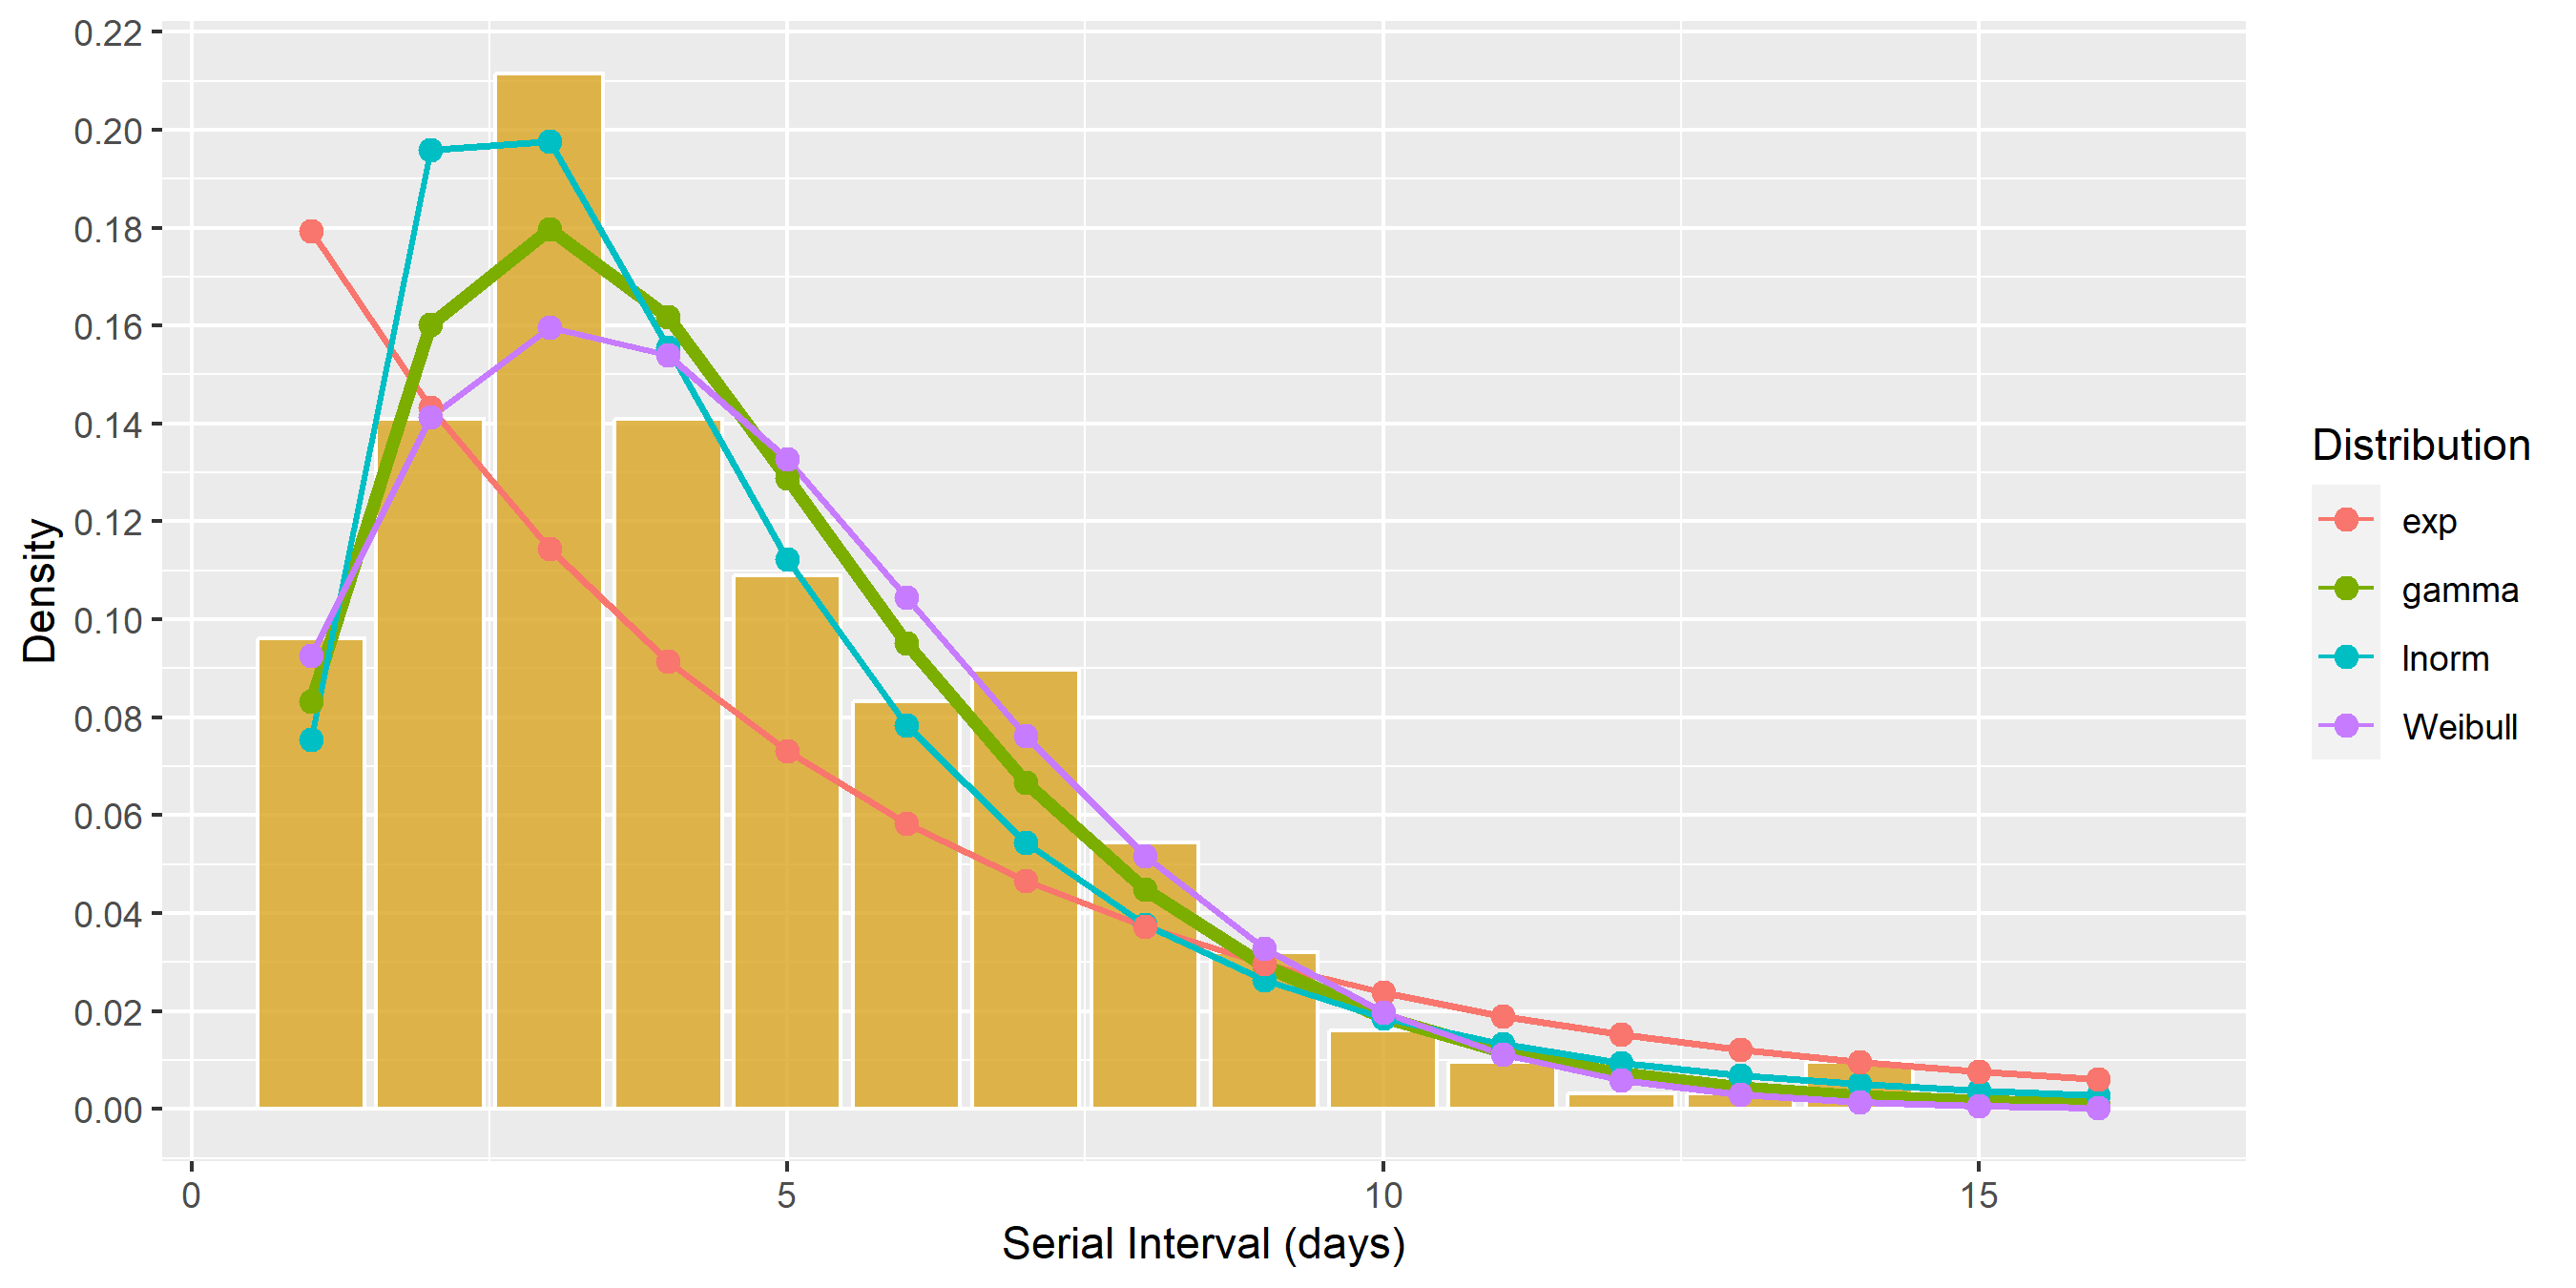
\includegraphics[width=0.75\textwidth,keepaspectratio]{img/fig2_fits_p1_2023-05-12.png}
  \caption{Empirical and fitted distributions of the serial interval of 312 Covid19 transmission pairs observed between 23.02.2020 and 01.04.2020, Austria. The gamma distribution which yields the best fit is highlighted with a thicker line.}
\end{figure}

\note{
Reasons for change:
\begin{itemize}
\item new variants
\item faster contact tracing $\Rightarrow$ faster isolation of cases
\item similar observations in e.g. UK
\end{itemize}
}
\end{frame}

\begin{frame}{SI estimates, 06.09.2020 -- 17.05.2021 (Alpha period)}
\protect\hypertarget{si-estimates-06.09.2020-17.05.2021-alpha-period}{}
\begin{minipage} {.70\textwidth}
\begin{figure}
  \centering
  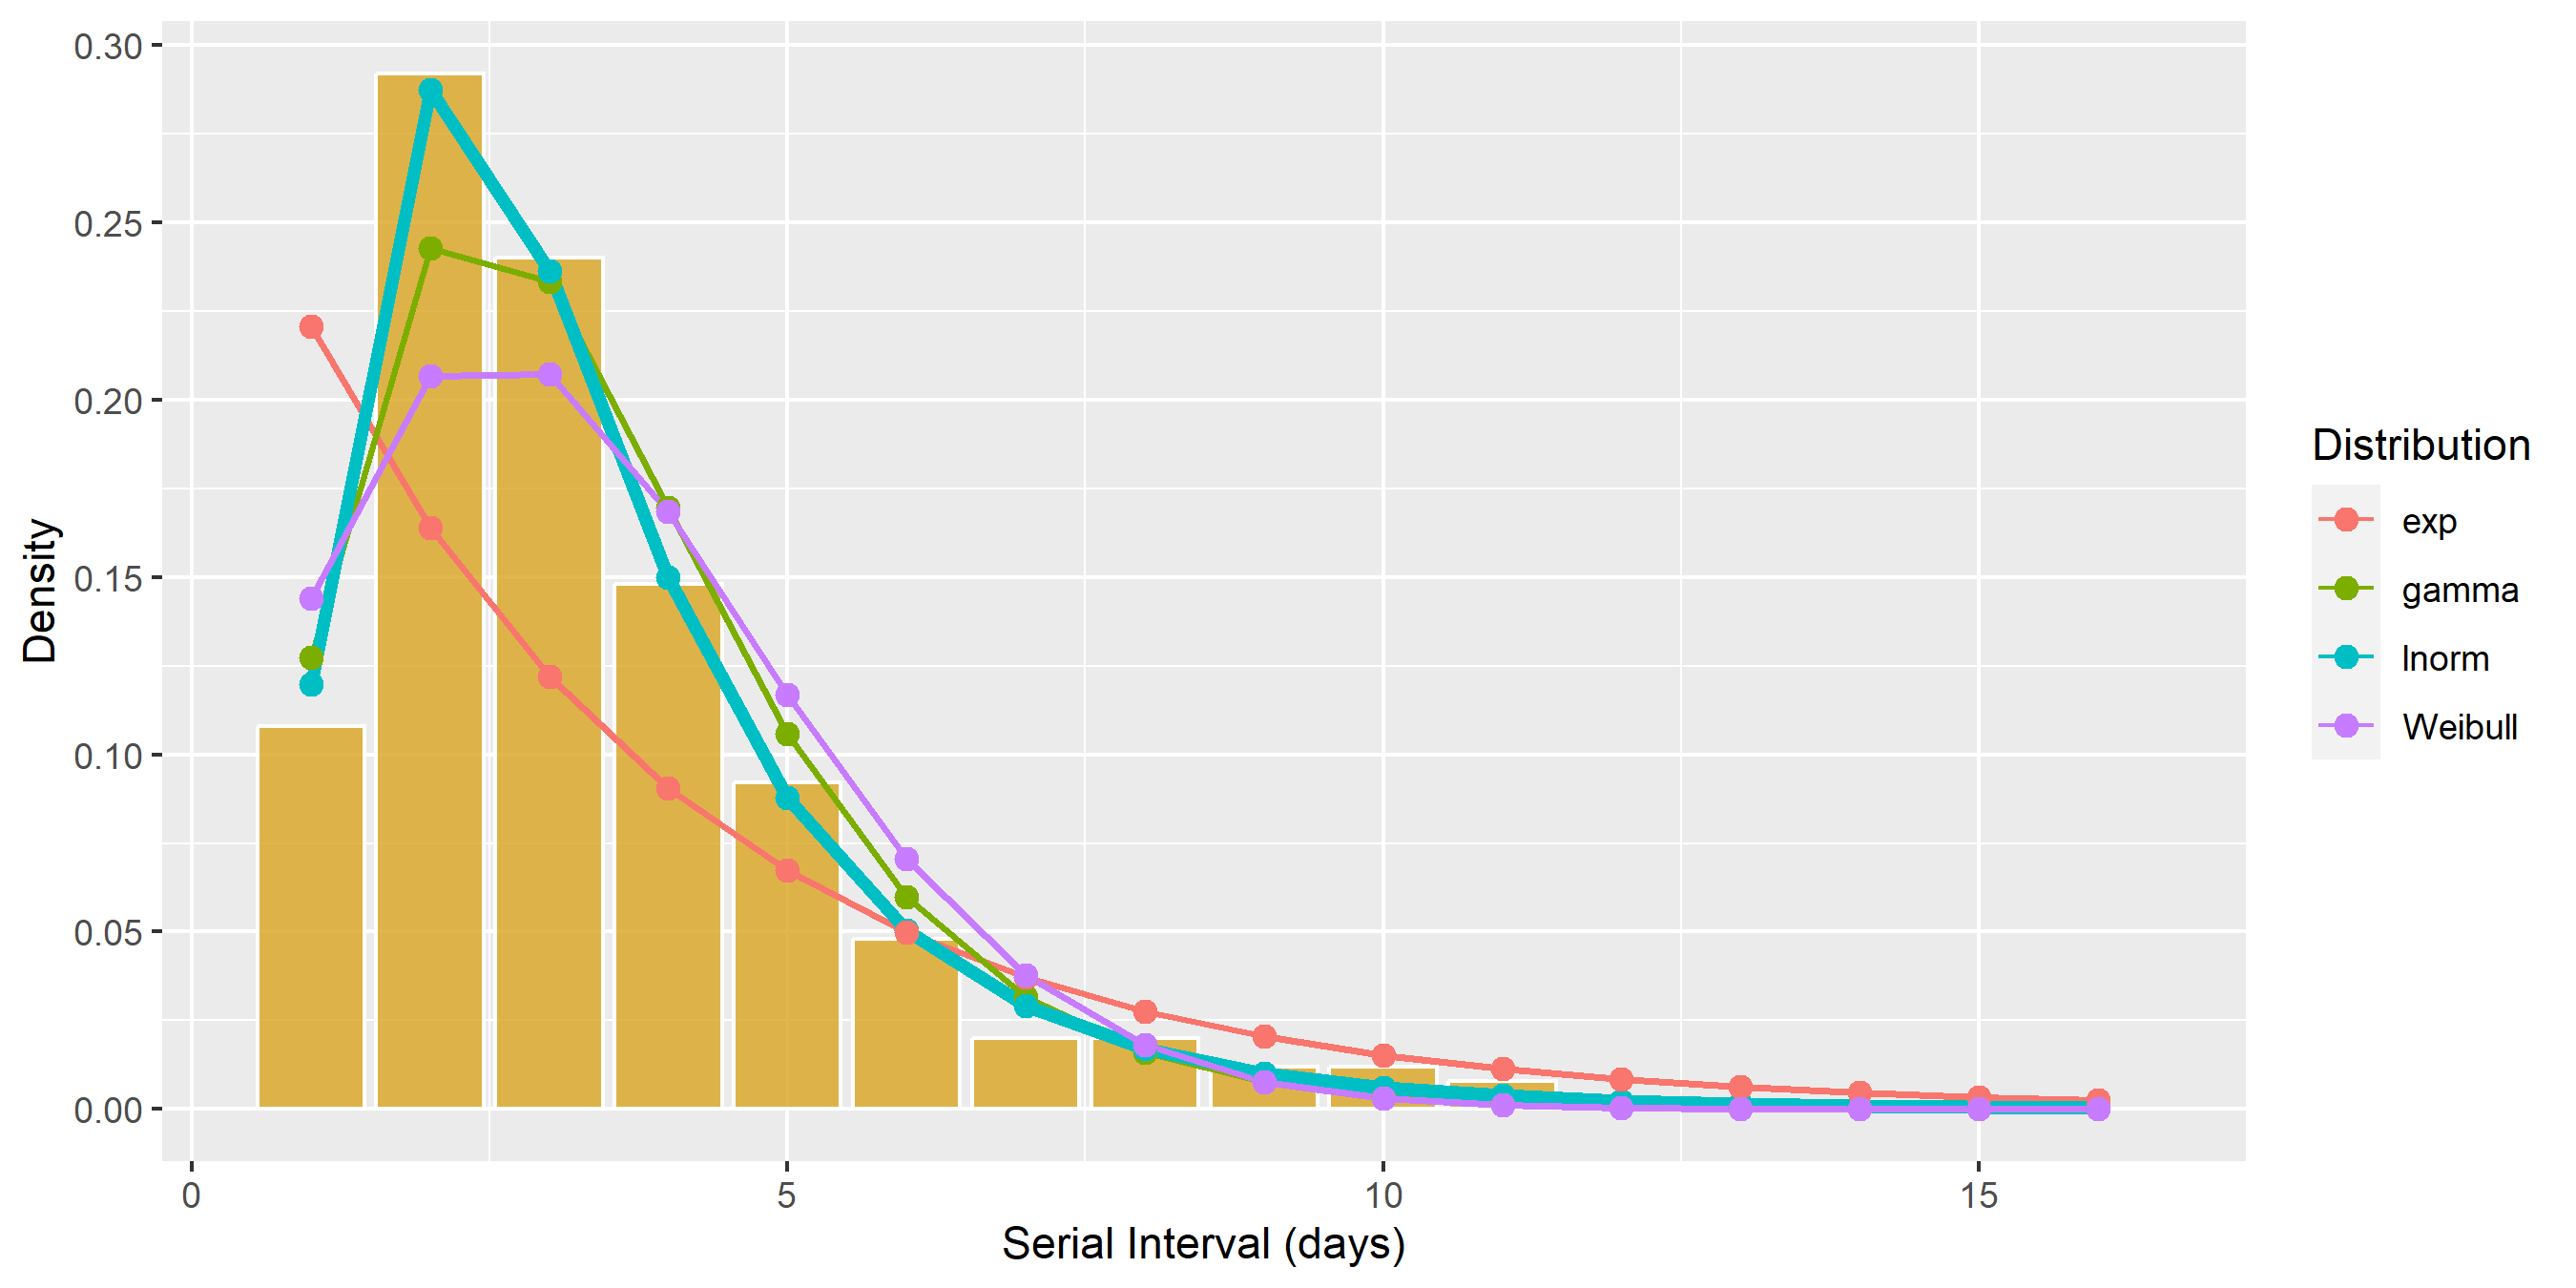
\includegraphics[width=0.8\textwidth,keepaspectratio]{img/fig2_fits_p2_2023-05-12.png}
  \caption{Empirical and fitted distributions of the serial interval of 250 Covid19 transmission pairs observed between 06.09.2020 and 17.05.2021, Austria. The lognormal  distribution which yields the best fit is highlighted with a thicker line.}
\end{figure}

\end{minipage}
\begin{minipage} {.25\textwidth}
\begin{itemize}
\item Mean of lnorm: \\ $3.38$ (95\% CI: $3.12$ -- $3.62$)
\item SD of lnorm: \\ $2.05$ (95\% CI: $1.74$ -- $2.37$)
\end{itemize}
\end{minipage}
\end{frame}

\begin{frame}{Basic and effective reproduction number}
\protect\hypertarget{basic-and-effective-reproduction-number}{}
\begin{block}{Definition $R_0$}
The basic reproduction number is the average number of secondary cases per infectious case in a population where \textbf{everyone is susceptible}. %\cite{Rothman2008}
\end{block}
\begin{block}{Definition $R_\mli{eff}$}
The effective reproduction number is the average number of secondary cases per infectious case in a population made up of both \textbf{susceptible and non-susceptible} hosts. %\cite{Rothman2008}
\end{block}
\pause
\begin{itemize}
\item $R_\mli{eff} > 1 \Rightarrow$ increasing number of cases.
\item $R_\mli{eff} = 1 \Rightarrow$ endemic transmission.
\item $R_\mli{eff} < 1 \Rightarrow$ decreasing number of cases.
\item Implicitly includes effects of interventions.
\end{itemize}
\end{frame}

\begin{frame}{\(R_\mli{eff}\), Cori Method (Cori et al.
(\protect\hyperlink{ref-cori2013}{2013}))}
\protect\hypertarget{r_mlieff-cori-method-cori2013}{}
\begin{itemize}
\item $y_t \sim Pois(\lambda_t)$, number of new cases at day $t$
\item $w_s$, probability that a case generates another case $s$ days after its infection
\item $s$, \underline{\textit{generation time}} with density $p(s;.)$
\item $s \approx SI$
\item For $s = 1, \dots, m$, $w_s = \frac{p(s;.)}{\sum_{i=1}^m p(i;.)}$ and $\sum_{i = 1}^m w_s = 1$
\item $R_\mli{eff}$ is the mean number of cases generated by one infected
\item Infected at time $t-s$ contribute with a rate of $R_\mli{eff}w_s$ to the number of cases at day $t$
\item cases at times $\{1,\dots, t-s-1, t-s+1,\dots, t-1\}$ also contribute to the number of cases at day $t$
\item $\lambda_t$ denotes the mean number of cases at day $t$, therefore $\lambda_t = R_\mli{eff} \sum_{s=1}^t y_{t-s}w_s$
\end{itemize}
\end{frame}

\begin{frame}{\(R_\mli{eff}\), Cori Method cont.}
\protect\hypertarget{r_mlieff-cori-method-cont.}{}
\begin{itemize}
\item Assumption: $R_\mli{eff}$ for day $t$ is constant over a period of $\tau$ days, hence we write $R_{t,\tau}$
\item Estimate $R_{t,\tau}$ using Bayesian inference
\begin{align*}
  R_{t,\tau} \sim \text{Gamma}\left(a+\sum_{i=t-\tau+1}^t y_i, \frac{1}{\frac{1}{b} + \sum_{i=t-\tau+1}^t \sum_{s=1}^i y_{i-s}w_s}\right)
\end{align*}
with $a$, $b$ parameters of the prior gamma distribution
\item Mean
\begin{align*}
  \hat{R}_{t,\tau} = \frac{a+\sum_{i=t-\tau+1}^t y_i}{\frac{1}{b} + \sum_{i=t-\tau+1}^t \sum_{s=1}^i y_{i-s}w_s}
\end{align*}
\item 95\% CI calculated as the 2.5\% and the 97.5\% percentile of the Gamma distribution 
\item \R{}-package \texttt{EpiEstim}
\end{itemize}
\end{frame}

\begin{frame}{RKI Method}
\protect\hypertarget{rki-method}{}
\begin{itemize}
\item Much simpler approach
\item $y_t$, number of incident cases at day $t$
\item $\tau$, number of days included in the estimation of $R_\mli{eff}$ as above
\item $s$, an integer denoting the generation time in full days
\item RKI estimate of $R_{t,\tau}$ is calculated as
\begin{align*}
  R_{t,\tau} = \frac{\sum_{i=t-\tau+1}^{t} y_t}{\sum_{i=t-\tau+1}^{t} y_{t-s}} = \frac{\bar{y}_t^\tau}{\bar{y}_{t-s}^\tau},
\end{align*}
where $\bar{y}_t^\tau = \frac{1}{\tau} \sum_{i=t-\tau+1}^{t} y_t$ is the moving average of cases of $\tau$ days. 
\end{itemize}
\end{frame}

\begin{frame}{Comparison of methods}
\protect\hypertarget{comparison-of-methods}{}
\begin{figure}
  \centering
  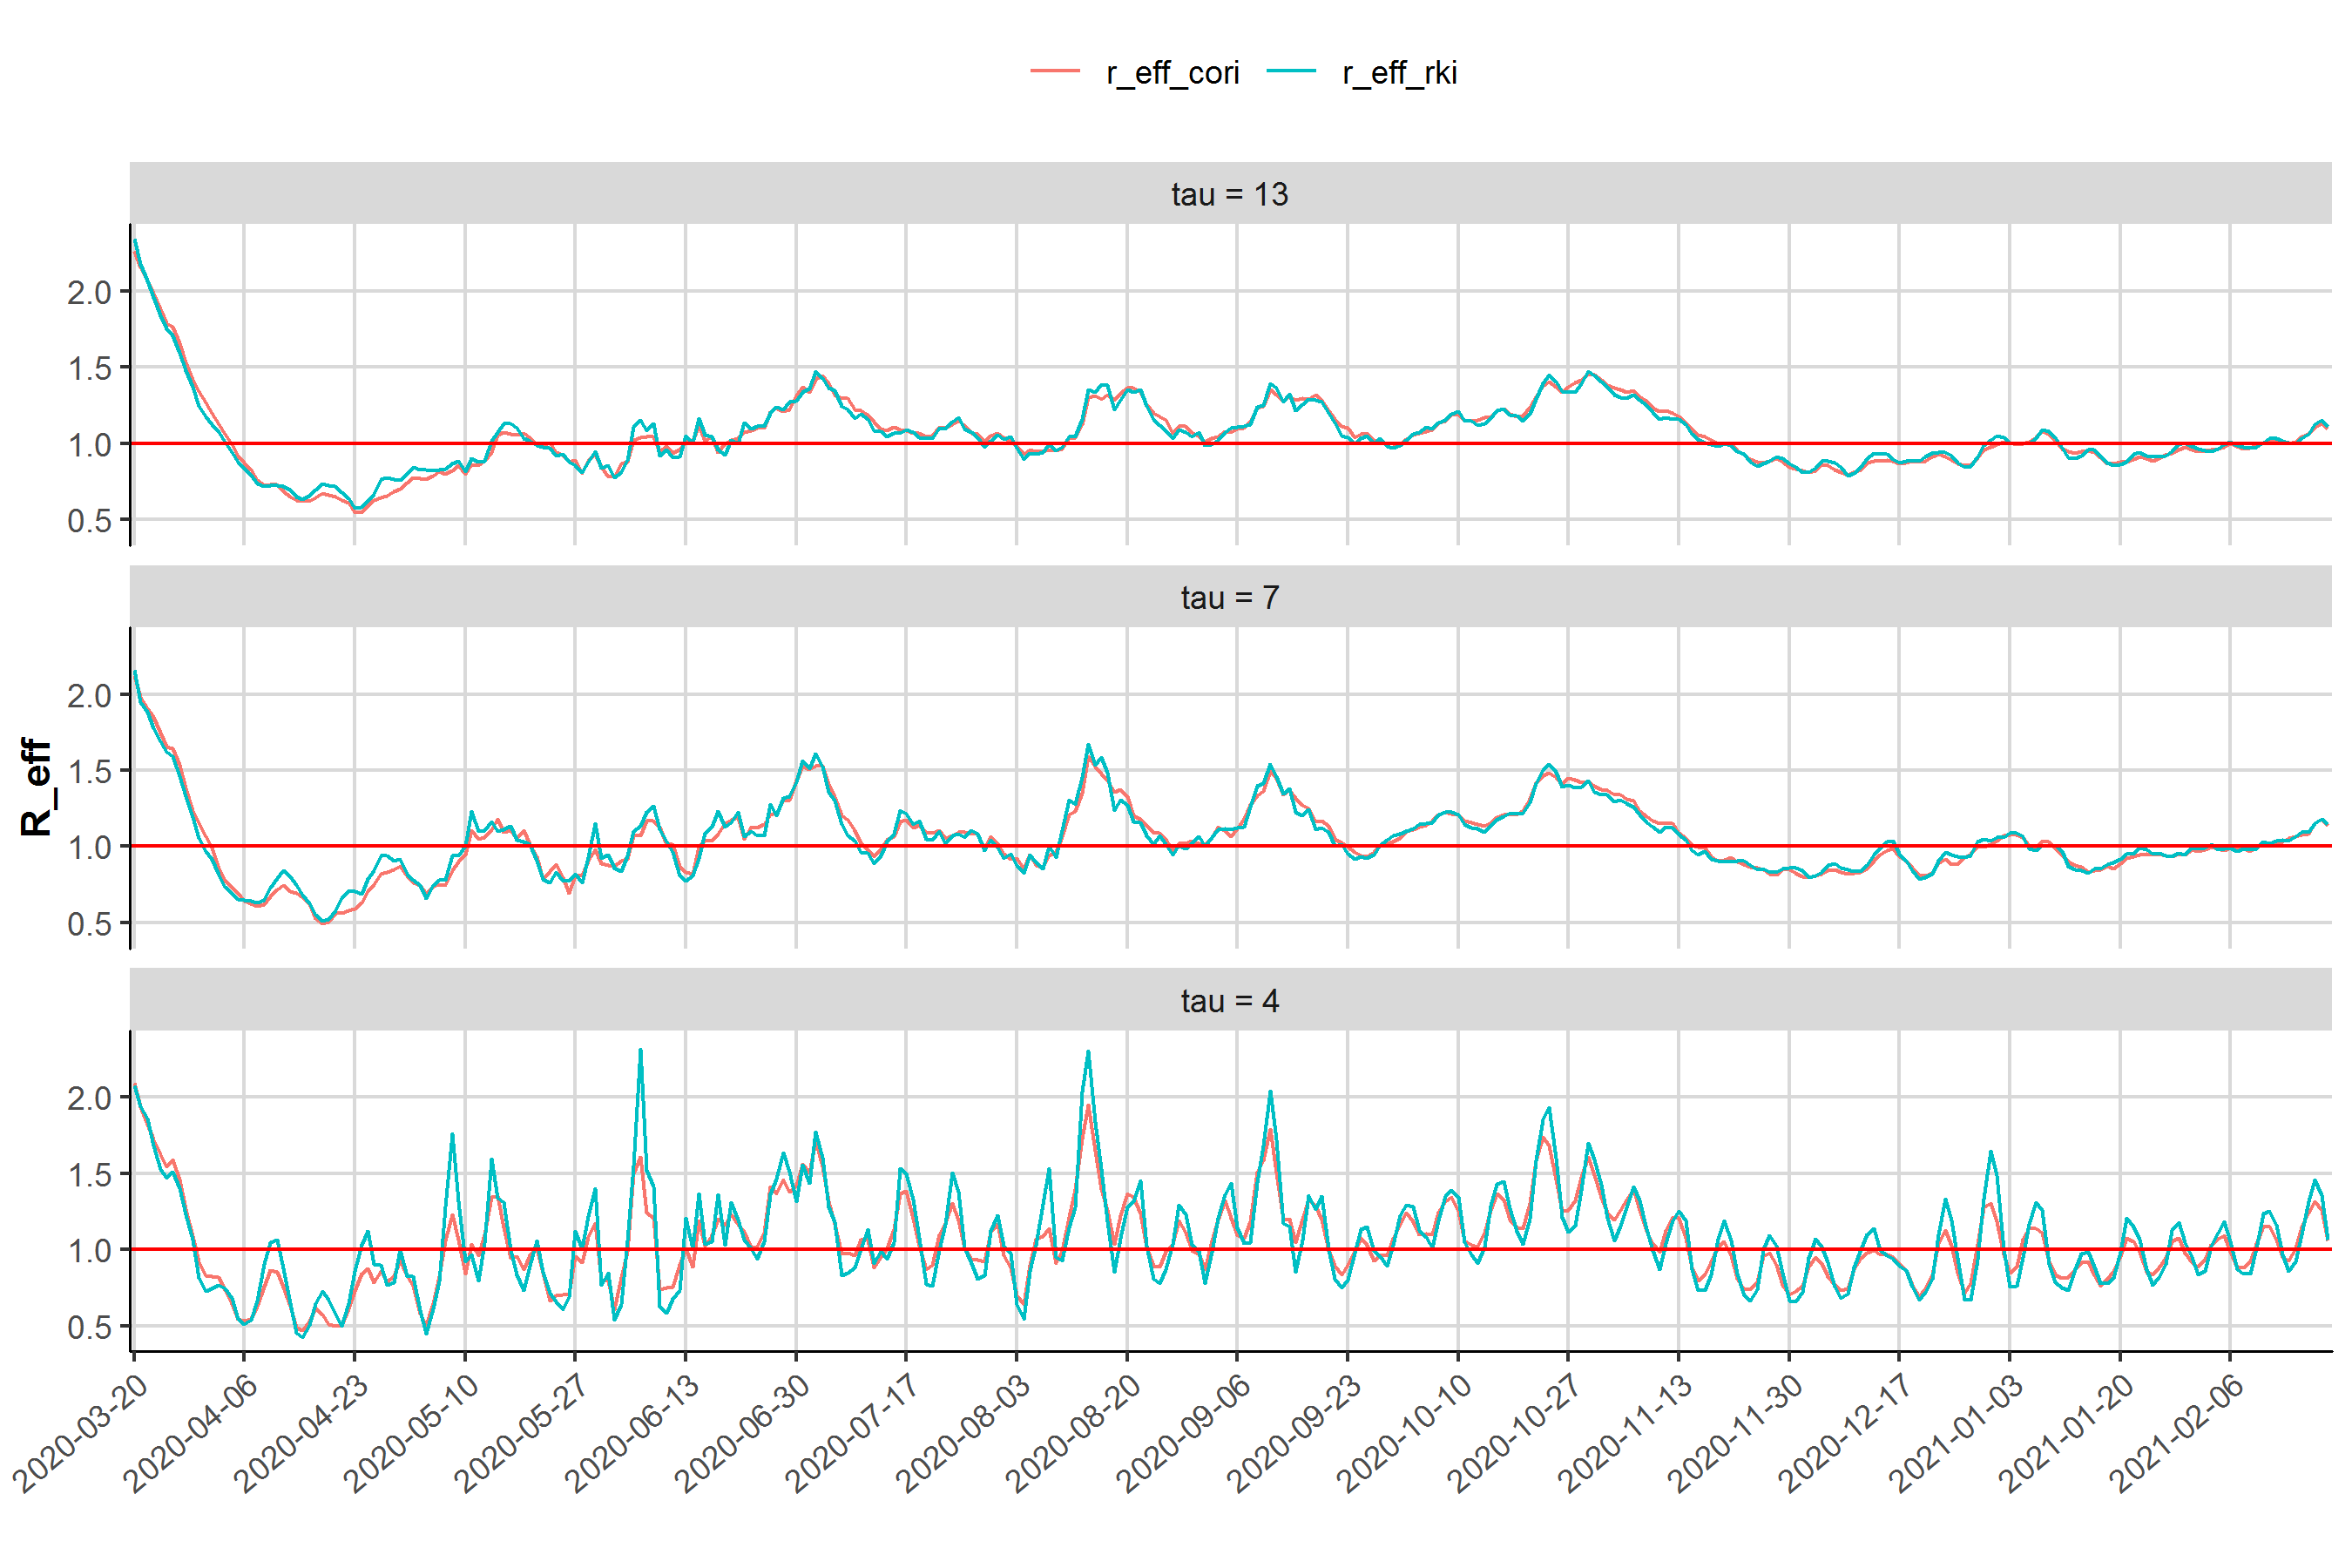
\includegraphics[height=0.8\textheight,keepaspectratio]{img/fig_r_eff_rki_cori_2021-02-23.png}
  \caption{Comparison of the effective reproduction number $R_{t,\tau}$ for the Cori and RKI method for different values of $\tau$.}
\end{figure}
\end{frame}

\begin{frame}{Imputation of date of onset}
\protect\hypertarget{imputation-of-date-of-onset}{}
\begin{itemize}
\tightlist
\item
  Date of onset is a key variable
\item
  Is often unknown \pause

  \begin{figure}
  \centering
  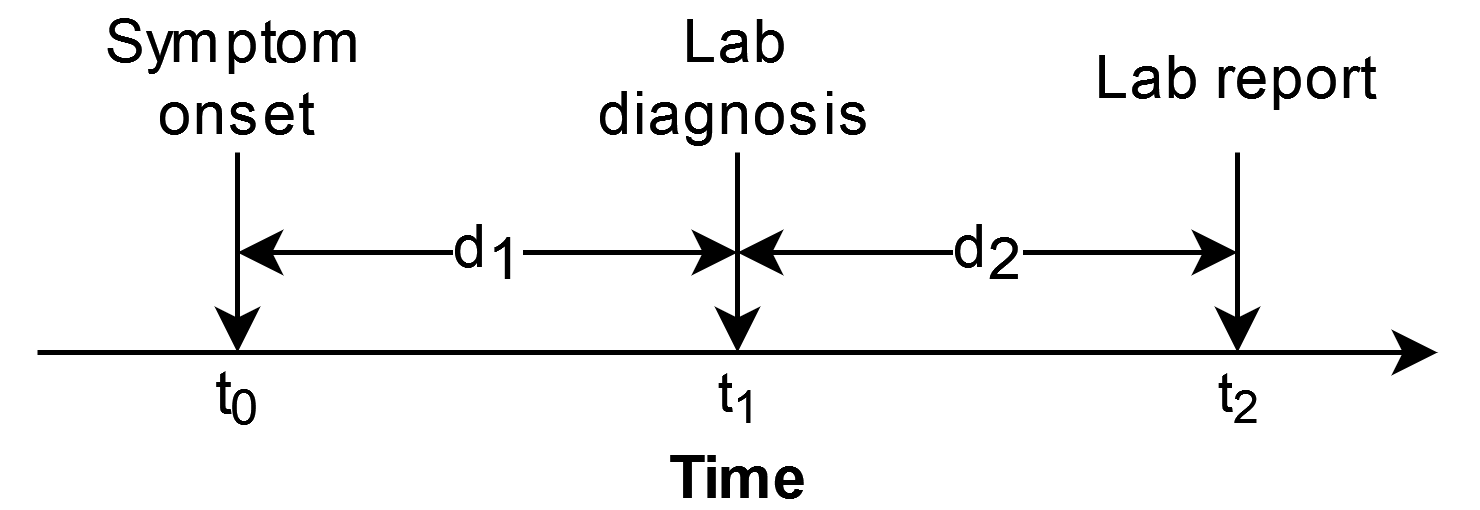
\includegraphics[width=0.5\textwidth,keepaspectratio]{img/reporting_delay_diagram.png}
  \caption{Diagram of the typical chronological order of a case from symptom onset to reporting.}
  \end{figure}
  \pause
\item
  date of reporting (\(t_2\)) vs.~date of onset (\(t_0\))
\item
  reporting delay: \(t_\mli{diff} := t_2 - t_0\)
\end{itemize}
\end{frame}

\begin{frame}{Imputation of date of onset II}
\protect\hypertarget{imputation-of-date-of-onset-ii}{}
\begin{itemize}
\tightlist
\item
  \(t_\mli{diff} \sim \text{Gamma}(\alpha, \beta),\, \alpha,\beta > 0.\)
\item
  PDF:
  \(p(y;\mu,\sigma) = \frac{y^{\frac{1}{\sigma^2}-1} \exp\left(-\frac{y}{\sigma^2 \mu}\right)}{(\sigma^2 \mu)^{\frac{1}{\sigma^2}} \Gamma\left(\frac{1}{\sigma^2}\right)}\)
  with \(\mu = \alpha / \beta\) and \(\sigma = 1 / \sqrt{\alpha}\)
\item
  \texttt{gamlss}-model
  (\textit{flexible generalized additive model for location, scale and shape})
  (Stasinopoulos and Rigby
  (\protect\hyperlink{ref-stasinopoulos2007}{2007})):
  \[\eta_{k,\mli{cw}} = \beta_{k,0} + \beta_{k,1} f(x_\mli{cw}), \, k \in \{\mu, \sigma\}\]
\item
  \(f(.)\), smoothing function (cubic splines)
\item
  \(x_\mli{cw}\), calendar week
\end{itemize}
\end{frame}

\begin{frame}{Results, 2020 week 9 to 22}
\protect\hypertarget{results-2020-week-9-to-22}{}
\begin{minipage}{.6\textwidth}

\setbeamerfont{caption}{size=\scriptsize}
\begin{figure}
  \centering
  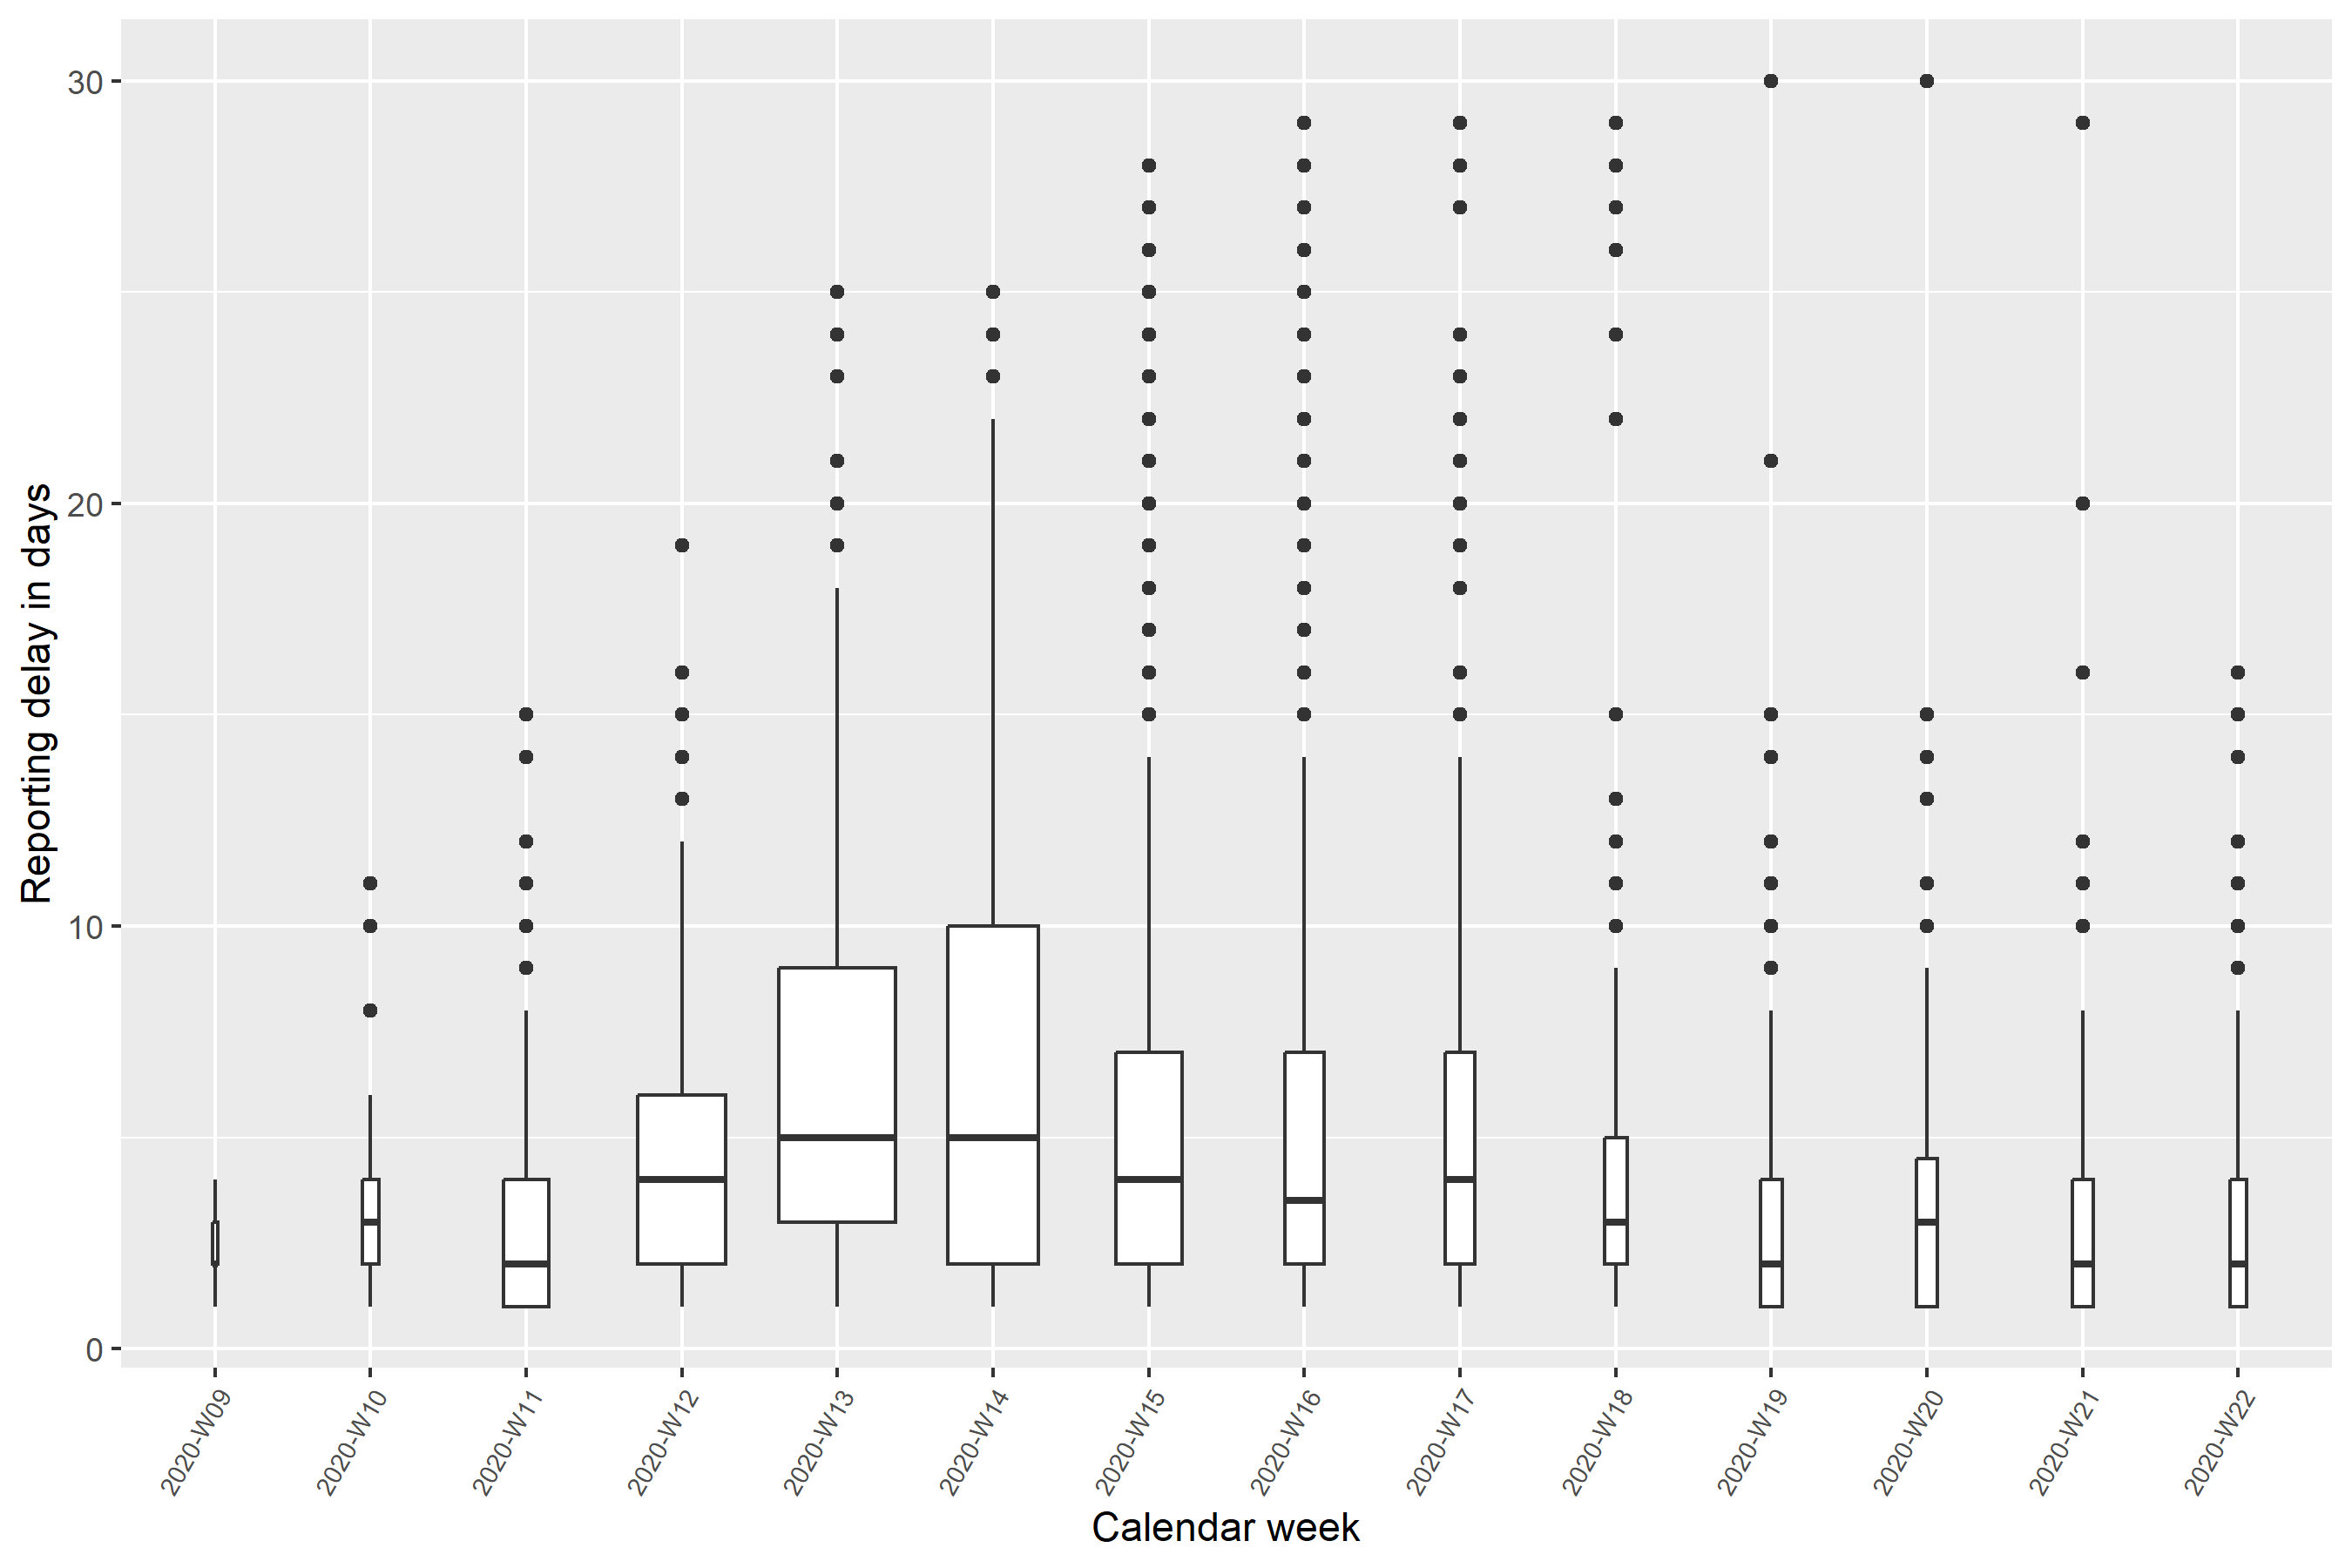
\includegraphics[width=0.9\textwidth,keepaspectratio]{img/reporting_delay_boxplot_phase1.png}
  \caption{Series of boxplots of the reporting delay $t_\mli{diff}$ by calendar week of cases with known date of report and date of disease onset of SARS-CoV-2, Austria, 2020 week 9 to week 22}
\end{figure}

\end{minipage}
\begin{minipage} {.37\textwidth}
\begin{itemize}
\item 16,878 cases
\item 12,027 (71.3\%) with reliable date of onset
\item weekly mean $t_\mli{diff}$ ranged from 2.38 -- 6.58
\end{itemize}

\setbeamerfont{caption}{size=\tiny}
\begin{table}
\centering 
\tiny
\caption{Parameter estimates of the \texttt{gamlss} model for $\hat{\mu}_\mli{cw}$ and $\hat{\sigma}_\mli{cw}$} 
\label{tab:gamlss_phase1} 
\begin{tabular}{@{\extracolsep{5pt}} crrr} 
\hline \\[-1.8ex] 
Parameter & Estimate & Std. Error & $p$ \\ 
\hline \\[-1.8ex] 
$\hat{\beta}_{\mu,0}$ & $1.474$ & $0.023$ & $<10^{-3}$ \\ 
$\hat{\beta}_{\mu,1}$ & $0.042$ & $0.004$ & $<10^{-3}$ \\ 
$\hat{\beta}_{\sigma,0}$ & $-0.519$ & $0.018$ & $<10^{-3}$ \\ 
$\hat{\beta}_{\sigma,1}$ & $0.044$ & $0.003$ & $<10^{-3}$ \\ 
\hline \\[-1.8ex] 
\end{tabular} 
\end{table}

\end{minipage}
\end{frame}

\begin{frame}{Epicurve and \(R_\mli{eff}\), 2020 week 9 to 22}
\protect\hypertarget{epicurve-and-r_mlieff-2020-week-9-to-22}{}
\begin{minipage}{.45\textwidth}

\setbeamerfont{caption}{size=\scriptsize}
\begin{figure}
  \centering
  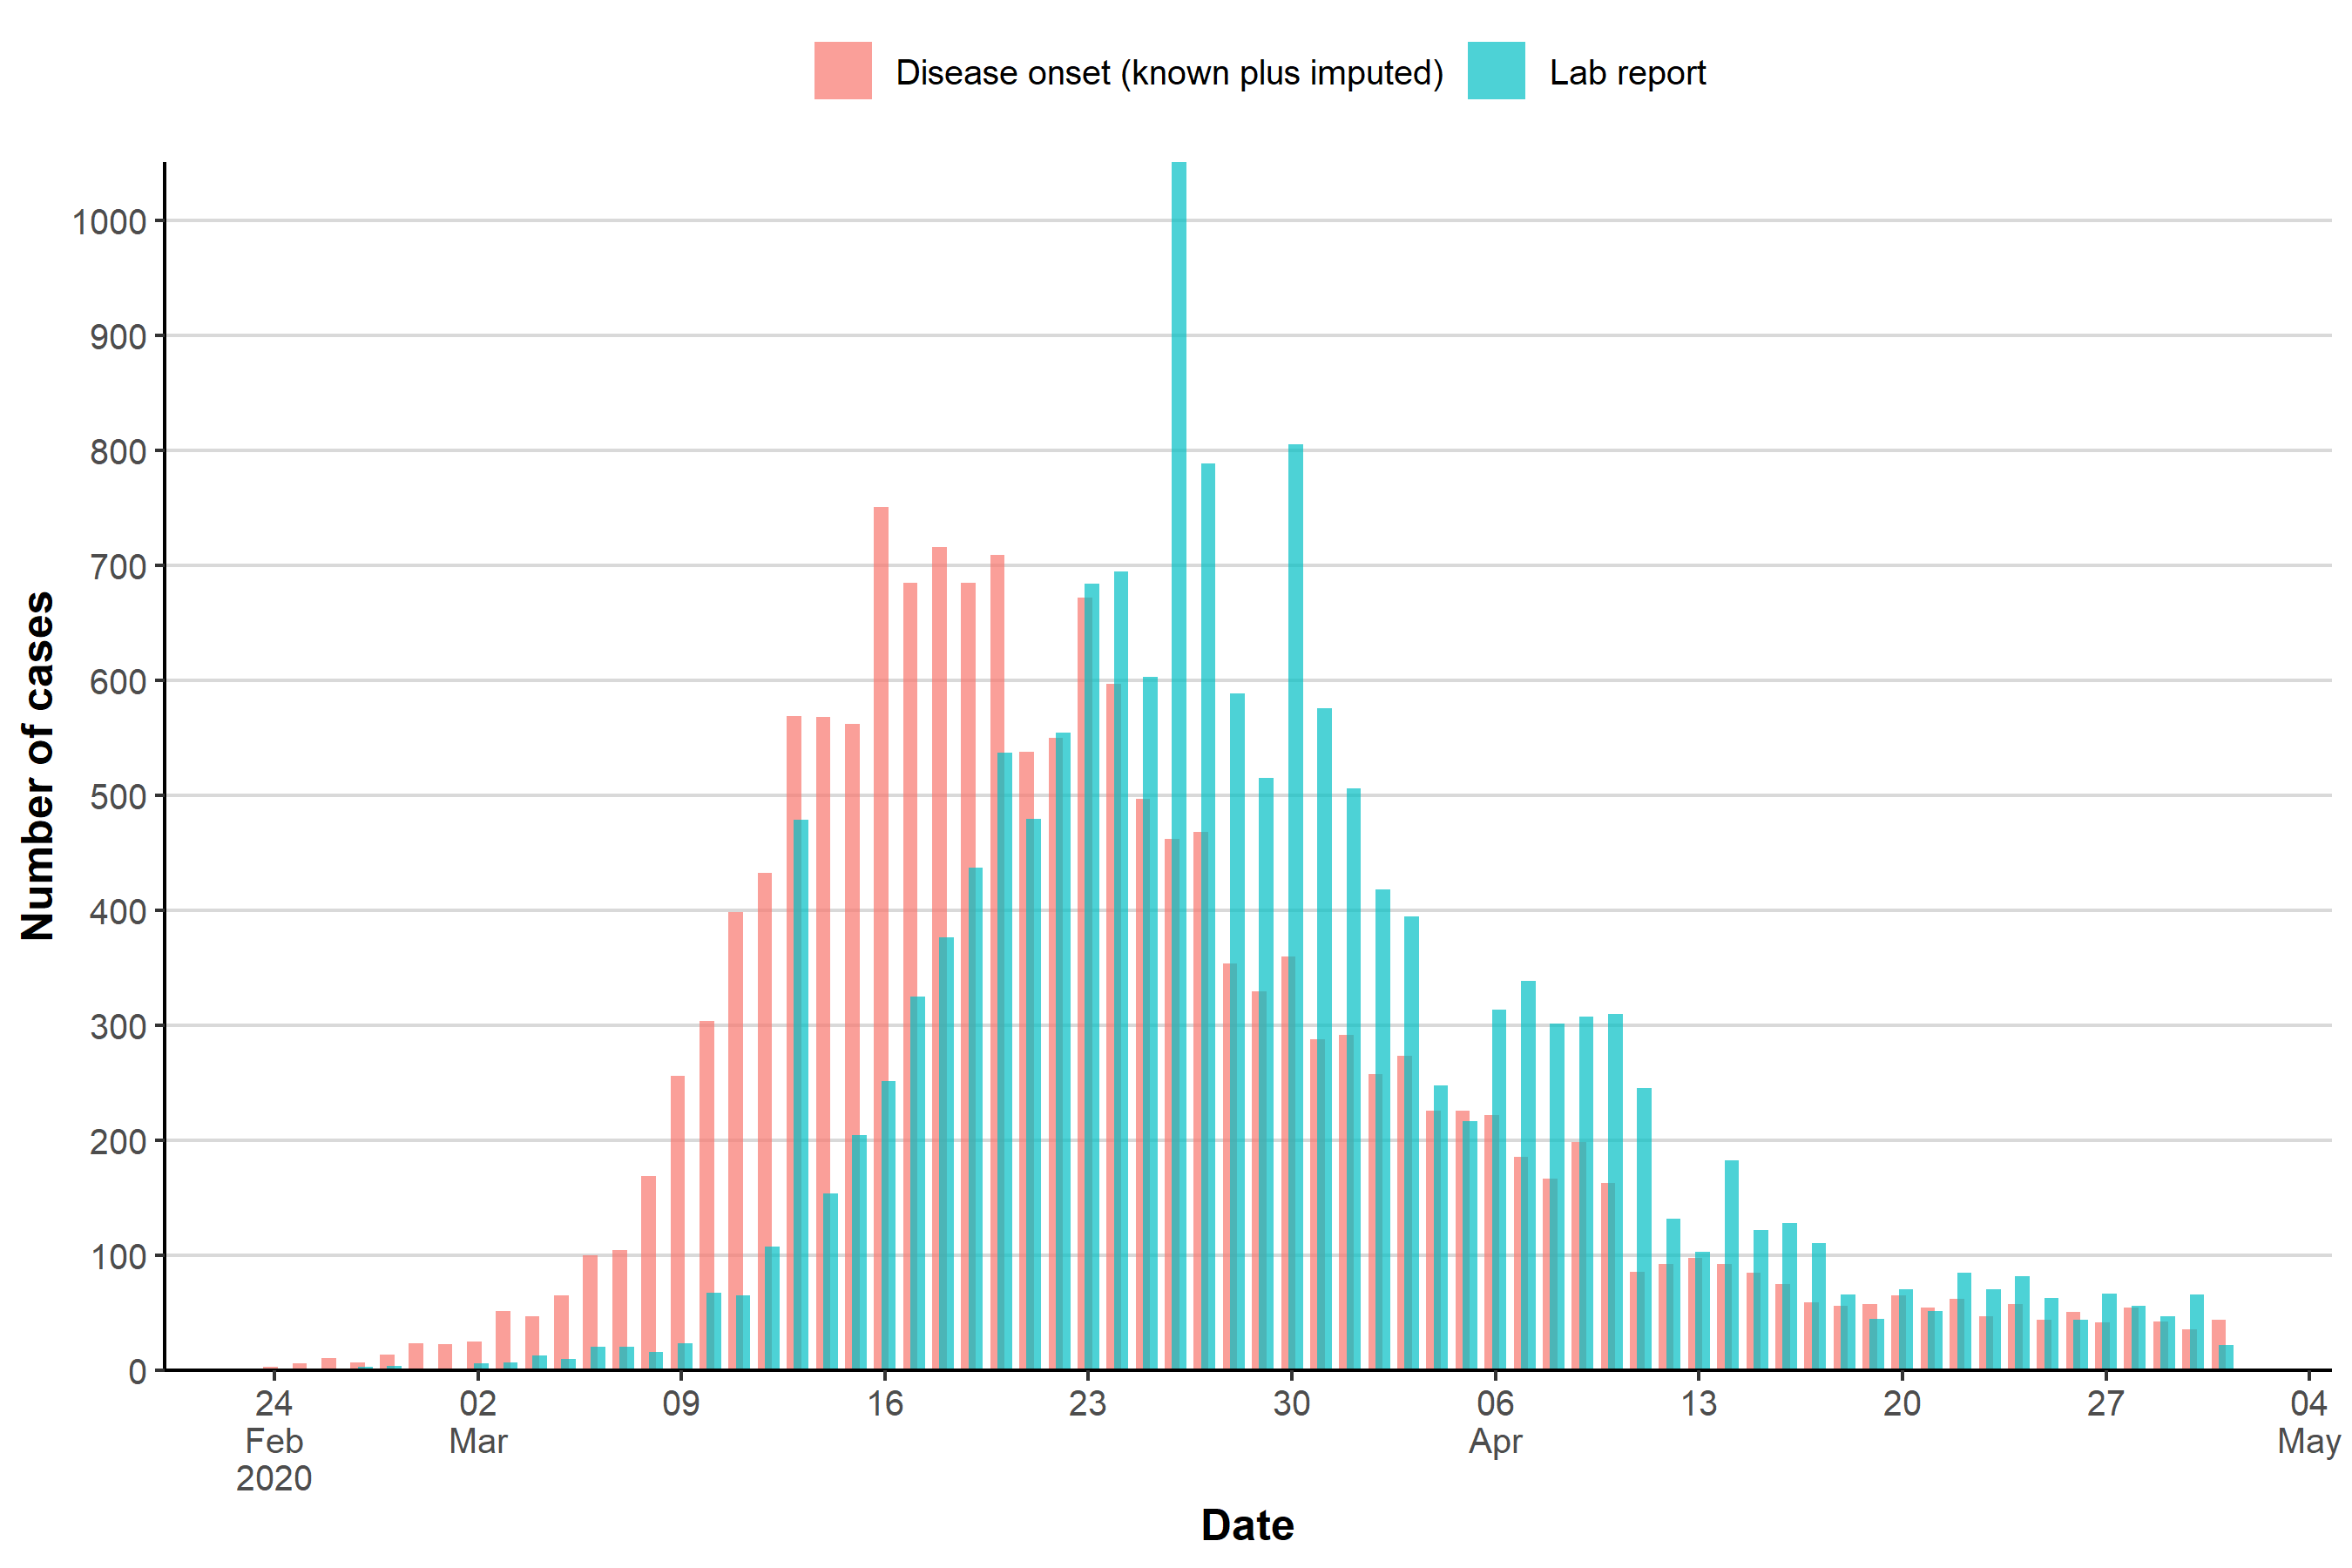
\includegraphics[width=0.95\textwidth,keepaspectratio]{img/epicurve_compare_imputed_phase1.png}
  \caption{Epicurve by date of disease onset (known and imputed) versus epicurve by date of lab report of SARS-CoV-2, Austria, 24.02.2020 (week 9) to 01.05.2020 (week 18)}
\end{figure}

\end{minipage}
\begin{minipage} {.45\textwidth}

\setbeamerfont{caption}{size=\scriptsize}
\begin{figure}
  \centering
  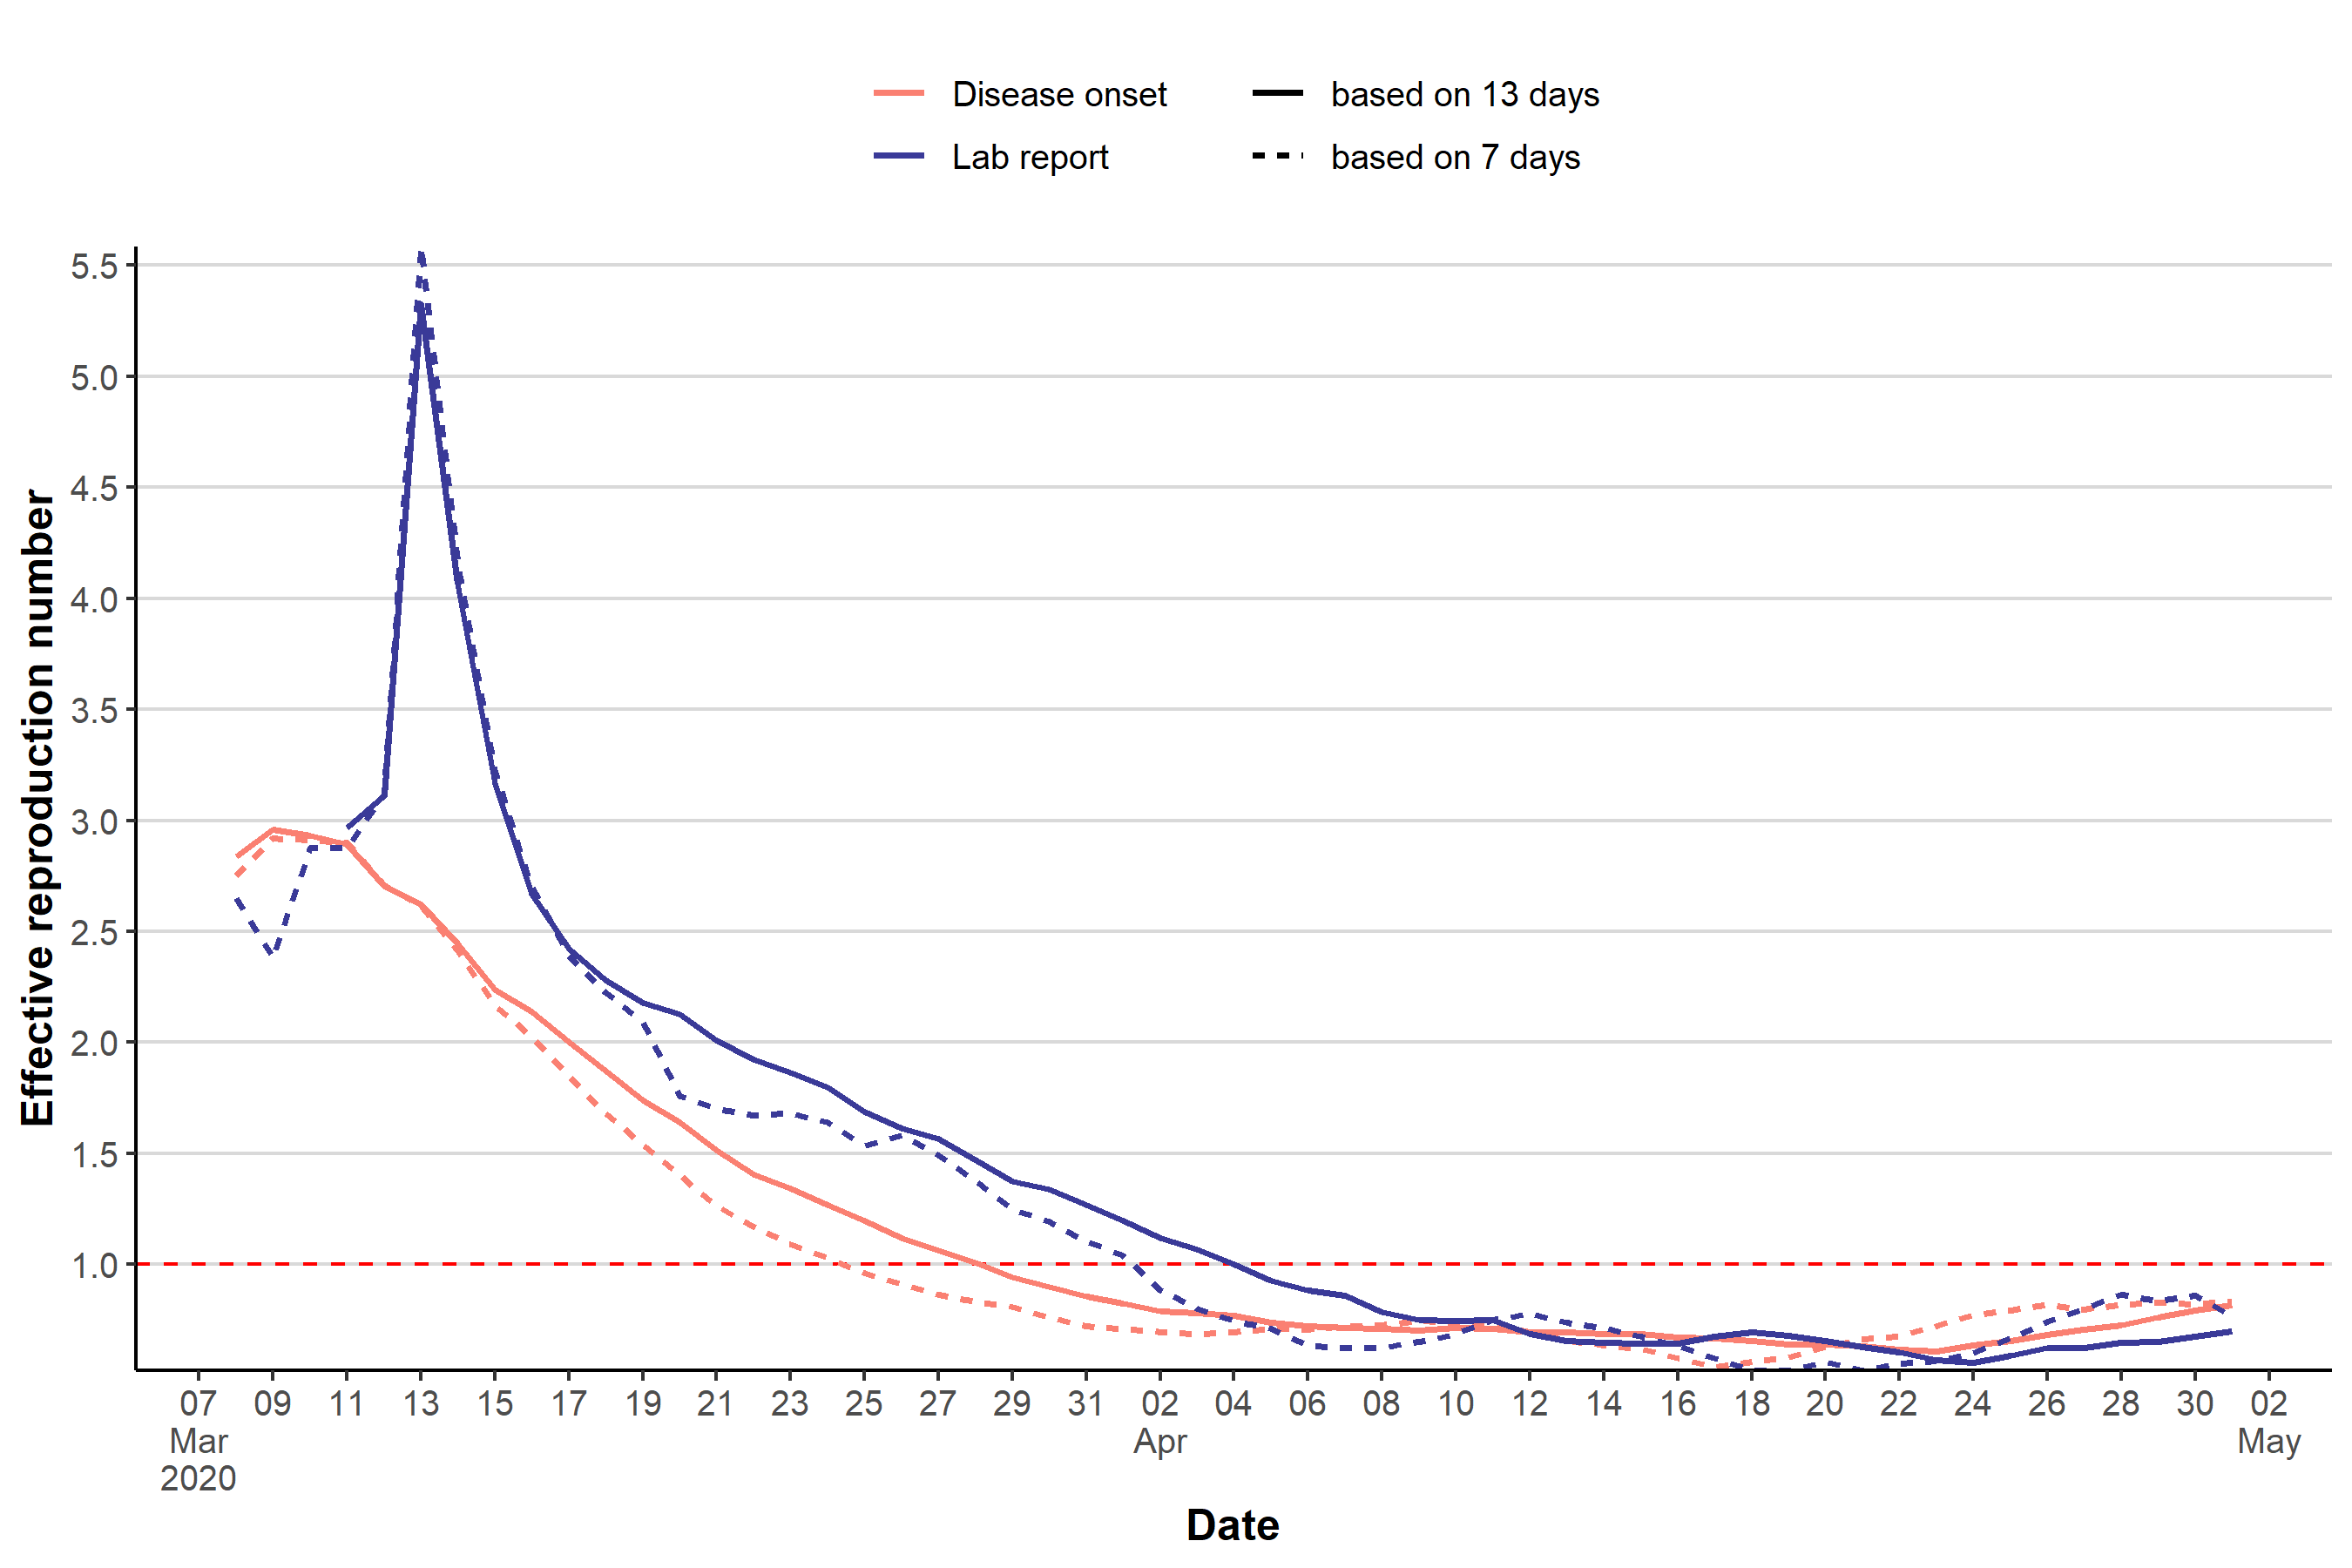
\includegraphics[width=0.95\textwidth,keepaspectratio]{img/r_eff_compare_phase1.png}
  \caption{Effective reproduction number based on date of disease onset (known and imputed, red) and based on date of lab report (blue) and based on different values of $\tau$ ($\tau = 13$ solid line, $\tau = 7$ days dashed line) of SARS-CoV-2 cases, Austria, 08.03.2020 (week 10) to 01.05.2020 (week 18)}
\end{figure}

\end{minipage}
\end{frame}

\begin{frame}{Imputation of variant data}
\protect\hypertarget{imputation-of-variant-data}{}
\begin{itemize}
\tightlist
\item
  December 2021 to January 2022: emergence of Omicron Variant
  (B.1.1.529)
\item
  Has mutation at the 501th segment of the genome: N501Y variant
\item
  We define

  \begin{itemize}
  \tightlist
  \item
    \(x_\mli{n501y} \in \{0,1,\mli{NA}\}\), a case has the N501Y
    mutation
  \item
    \(x_\mli{omicron} \in \{0,1,\mli{NA}\}\), a case has the Omicron
    variant
  \end{itemize}
\item
  Two-stage imputation
\end{itemize}

\pause

A case can enter one of four states:

\begin{enumerate}
  \item $x_\mli{n501y}=\mli{NA} \Rightarrow x_\mli{omicron}=\mli{NA}$
  \item $x_\mli{n501y}=0 \Rightarrow x_\mli{omicron}=0$
  \item $x_\mli{n501y}=1$ and $x_\mli{omicron}=\mli{NA}$
  \item $x_\mli{n501y}=1$ and $x_\mli{omicron} \in \{0,1\}$
\end{enumerate}
\end{frame}

\begin{frame}{Modelling \(x_\mli{n501y}\) and \(x_\mli{omicron}\)}
\protect\hypertarget{modelling-x_mlin501y-and-x_mliomicron}{}
\begin{itemize}
\item
  \(x_\mli{n501y} \sim \text{Bernoulli}(r)\)
\item
  standardised binomial model using province, calendar week and day of
  week as explanatory variables:
  \[logit(r) = \beta_0 + \beta_1 x_\mli{cw} + \beta_2 x_\mli{prov} + \beta_3 x_\mli{dow} + \varepsilon\]
  \pause
\item
  From above: \(x_\mli{n501y}=0 \Rightarrow x_\mli{omicron}=0\) and if
  \(x_\mli{n501y}=1 \Rightarrow x_\mli{omicron} \sim \text{Bernoulli}(s)\)
\item
  Analogously
  \[logit(s) = \gamma_0 + \gamma_1 x_\mli{cw} + \gamma_2 x_\mli{prov} + \gamma_3 x_\mli{dow} + \varepsilon\]
\end{itemize}
\end{frame}

\begin{frame}{Imputation of missing data}
\protect\hypertarget{imputation-of-missing-data}{}
\begin{itemize}
\tightlist
\item
  Impute missing values of \(\hat{x}_\mli{omicron}\) where
  \(x_\mli{n501y}\) is known by randomly imputing binary values based
  on: \begin{align*}
  \begin{split}
  P(\hat{x}_\mli{omicron}=1|x_\mli{n501y}=1)&=\hat{s},\\ P(\hat{x}_\mli{omicron}=0|x_\mli{n501y}=1)&=1-\hat{s},\\
  P(\hat{x}_\mli{omicron}=0|x_\mli{n501y}=0)&=1 \text{ and }\\ P(\hat{x}_\mli{omicron}=1|x_\mli{n501y}=0)&=0.
  \end{split}
  \end{align*} \pause
\item
  Randomly impute \(\hat{x}_\mli{n501y}\) and \(\hat{x}_\mli{omicron}\)
  for cases with \(x_\mli{n501y}=\mli{NA}\) and
  \(x_\mli{omicron}=\mli{NA}\) based on: \begin{align*}
  P(\hat{x}_\mli{omicron} = 0, \hat{x}_\mli{n501y} = 0) = P(\hat{x}_\mli{omicron} = 0 | \hat{x}_\mli{n501y} = 0)P(\hat{x}_\mli{n501y} = 0) &= 1 - \hat{r}, \\
  P(\hat{x}_\mli{omicron} = 0, \hat{x}_\mli{n501y} = 1) = P(\hat{x}_\mli{omicron} = 0 | \hat{x}_\mli{n501y} = 1)P(\hat{x}_\mli{n501y} = 1) &= (1 - \hat{s}) \hat{r}, \\
  P(\hat{x}_\mli{omicron} = 1, \hat{x}_\mli{n501y} = 1) = P(\hat{x}_\mli{omicron} = 1 | \hat{x}_\mli{n501y} = 1)P(\hat{x}_\mli{n501y} = 1) &= \hat{s}\hat{r}.
  \end{align*}
\end{itemize}
\end{frame}

\begin{frame}{Summary of cases for variant imputation}
\protect\hypertarget{summary-of-cases-for-variant-imputation}{}
\begin{table}
\caption{Summary of SARS-CoV-2 cases during the emergence of the Omicron variant, Austria,  22.11.2021 to 14.02.2022}
\centering
\begin{tabular}[t]{>{\raggedright\arraybackslash}p{7cm}rr}
\toprule
\textbf{} & \textbf{$n$} & \textbf{\% of total cases}\\
\midrule
\cellcolor{gray!6}{Total cases} & \cellcolor{gray!6}{1,253,256} & \cellcolor{gray!6}{100.0\%}\\
N501Y status and variant known & 348,727 & 27.8\%\\
\cellcolor{gray!6}{N501Y status known and variant unknown} & \cellcolor{gray!6}{1,038} & \cellcolor{gray!6}{0.1\%}\\
N501Y and variant unknown & 903,491 & 72.1\%\\
\midrule
\cellcolor{gray!6}{Other variant known} & \cellcolor{gray!6}{68,786} & \cellcolor{gray!6}{5.5\%}\\
Omicron variant known & 279,941 & 22.3\%\\
\cellcolor{gray!6}{Other variant imputed} & \cellcolor{gray!6}{154,364} & \cellcolor{gray!6}{12.3\%}\\
Omicron variant imputed & 750,165 & 59.9\%\\
\midrule
\cellcolor{gray!6}{cases with variant data imputed} & \cellcolor{gray!6}{904,529} & \cellcolor{gray!6}{72.2\%}\\
\bottomrule
\end{tabular}
\end{table}
\end{frame}

\begin{frame}{Model results}
\protect\hypertarget{model-results}{}
\begin{minipage}{.60\textwidth}

\setbeamerfont{caption}{size=\tiny}
\begin{table}[!htbp] \centering 
\tiny
  \caption{Binomial model estimates for $r$ (being N501Y) and $s$ (being Omicron), 22.11.2021 to 14.02.2022} 
\begin{tabular}{@{\extracolsep{5pt}}lcc} 
\\[-1.8ex]\hline 
\hline \\[-1.8ex] 
 & \multicolumn{2}{c}{\textit{Dependent variable:}} \\ 
\cline{2-3} 
\\[-1.8ex] & $r$ & $s$ \\ 
\\[-1.8ex] & (1) & (2)\\ 
\hline \\[-1.8ex] 
 kw & 1.269$^{***}$ (0.006) & $-$0.016 (0.015) \\ 
  dow2 & 0.299$^{***}$ (0.030) & 0.197$^{**}$ (0.089) \\ 
  dow3 & 0.475$^{***}$ (0.032) & 0.008 (0.088) \\ 
  dow4 & 0.574$^{***}$ (0.032) & 0.179$^{**}$ (0.089) \\ 
  dow5 & 0.726$^{***}$ (0.033) & 0.212$^{**}$ (0.091) \\ 
  dow6 & 0.864$^{***}$ (0.034) & 0.473$^{***}$ (0.107) \\ 
  dow7 & 0.994$^{***}$ (0.033) & 0.466$^{***}$ (0.108) \\ 
  blKärnten & $-$0.493$^{***}$ (0.062) &  \\ 
  blNiederösterreich & $-$0.337$^{***}$ (0.056) &  \\ 
  blOberösterreich & $-$0.491$^{***}$ (0.055) &  \\ 
  blSalzburg & 0.839$^{***}$ (0.059) &  \\ 
  blSteiermark & $-$0.112$^{*}$ (0.062) &  \\ 
  blTirol & 0.181$^{***}$ (0.057) &  \\ 
  blVorarlberg & $-$0.375$^{***}$ (0.065) &  \\ 
  blWien & 0.302$^{***}$ (0.053) &  \\ 
  Constant & $-$124.557$^{***}$ (0.555) & 6.602$^{***}$ (1.479) \\ 
 \hline \\[-1.8ex] 
Observations & 347,181 & 281,511 \\ 
Log Likelihood & $-$48,455.860 & $-$9,701.072 \\ 
Akaike Inf. Crit. & 96,943.710 & 19,418.140 \\ 
\hline 
\hline \\[-1.8ex] 
\textit{Note:}  & \multicolumn{2}{r}{$^{*}$p$<$0.1; $^{**}$p$<$0.05; $^{***}$p$<$0.01} \\ 
\end{tabular} 
\end{table}

\end{minipage}
\begin{minipage}{.30\textwidth}

\begin{itemize}
\item Very few ($\le 10$) non-Omicron cases among N501Y cases for 4 of 9 provinces
\item $x_\mli{prov}$ omitted from model for $s$
\item Almost all variables are significant
\begin{itemize}
\item Sample size effect?
\end{itemize}
\end{itemize}

\end{minipage}
\end{frame}

\begin{frame}{Model results of a subset}
\protect\hypertarget{model-results-of-a-subset}{}
\setbeamerfont{caption}{size=\tiny}
\begin{minipage}{.60\textwidth}

\begin{table}[!htbp] \centering 
\tiny
  \caption{Subset: Binomial model estimates for $r$ (being N501Y) and $s$ (being Omicron), 22.11.2021 to 14.02.2022} 
\begin{tabular}{@{\extracolsep{5pt}}lcc} 
\\[-1.8ex]\hline 
\hline \\[-1.8ex] 
 & \multicolumn{2}{c}{\textit{Dependent variable:}} \\ 
\cline{2-3} 
\\[-1.8ex] & $r$ & $s$ \\ 
\\[-1.8ex] & (1) & (2)\\ 
\hline \\[-1.8ex] 
 kw & 1.276$^{***}$ (0.041) & $-$0.027 (0.097) \\ 
  dow2 & 0.224 (0.232) & $-$0.496 (0.710) \\ 
  dow3 & 0.341 (0.232) & $-$0.881 (0.681) \\ 
  dow4 & 0.029 (0.224) & 0.627 (0.914) \\ 
  dow5 & 0.597$^{**}$ (0.238) & $-$0.624 (0.693) \\ 
  dow6 & 0.666$^{***}$ (0.245) & $-$0.903 (0.713) \\ 
  dow7 & 1.127$^{***}$ (0.254) & $-$0.468 (0.772) \\ 
  blKärnten & $-$0.988$^{**}$ (0.442) &  \\ 
  blNiederösterreich & $-$0.528 (0.410) &  \\ 
  blOberösterreich & $-$0.637 (0.402) &  \\ 
  blSalzburg & 0.497 (0.421) &  \\ 
  blSteiermark & 0.122 (0.463) &  \\ 
  blTirol & $-$0.305 (0.412) &  \\ 
  blVorarlberg & $-$0.802$^{*}$ (0.481) &  \\ 
  blWien & $-$0.037 (0.389) &  \\ 
  Constant & $-$124.853$^{***}$ (4.042) & 8.266 (9.931) \\ 
 \hline \\[-1.8ex] 
Observations & 6,667 & 5,445 \\ 
Log Likelihood & $-$948.006 & $-$213.260 \\ 
Akaike Inf. Crit. & 1,928.012 & 442.519 \\ 
\hline 
\hline \\[-1.8ex] 
\textit{Note:}  & \multicolumn{2}{r}{$^{*}$p$<$0.1; $^{**}$p$<$0.05; $^{***}$p$<$0.01} \\ 
\end{tabular} 
\end{table}

\end{minipage}
\begin{minipage}{.30\textwidth}

\begin{itemize}
\item Random sample of 23,658 cases
\item Much less significant variables
\item Model estimates: full vs. subset?
\end{itemize}

\end{minipage}
\end{frame}

\begin{frame}{Model estimates full (red) vs.~1000 samples, model of
\(r\)}
\protect\hypertarget{model-estimates-full-red-vs.-1000-samples-model-of-r}{}
\begin{minipage}{.60\textwidth}
\setbeamerfont{caption}{size=\scriptsize}
\begin{figure}
  \centering
  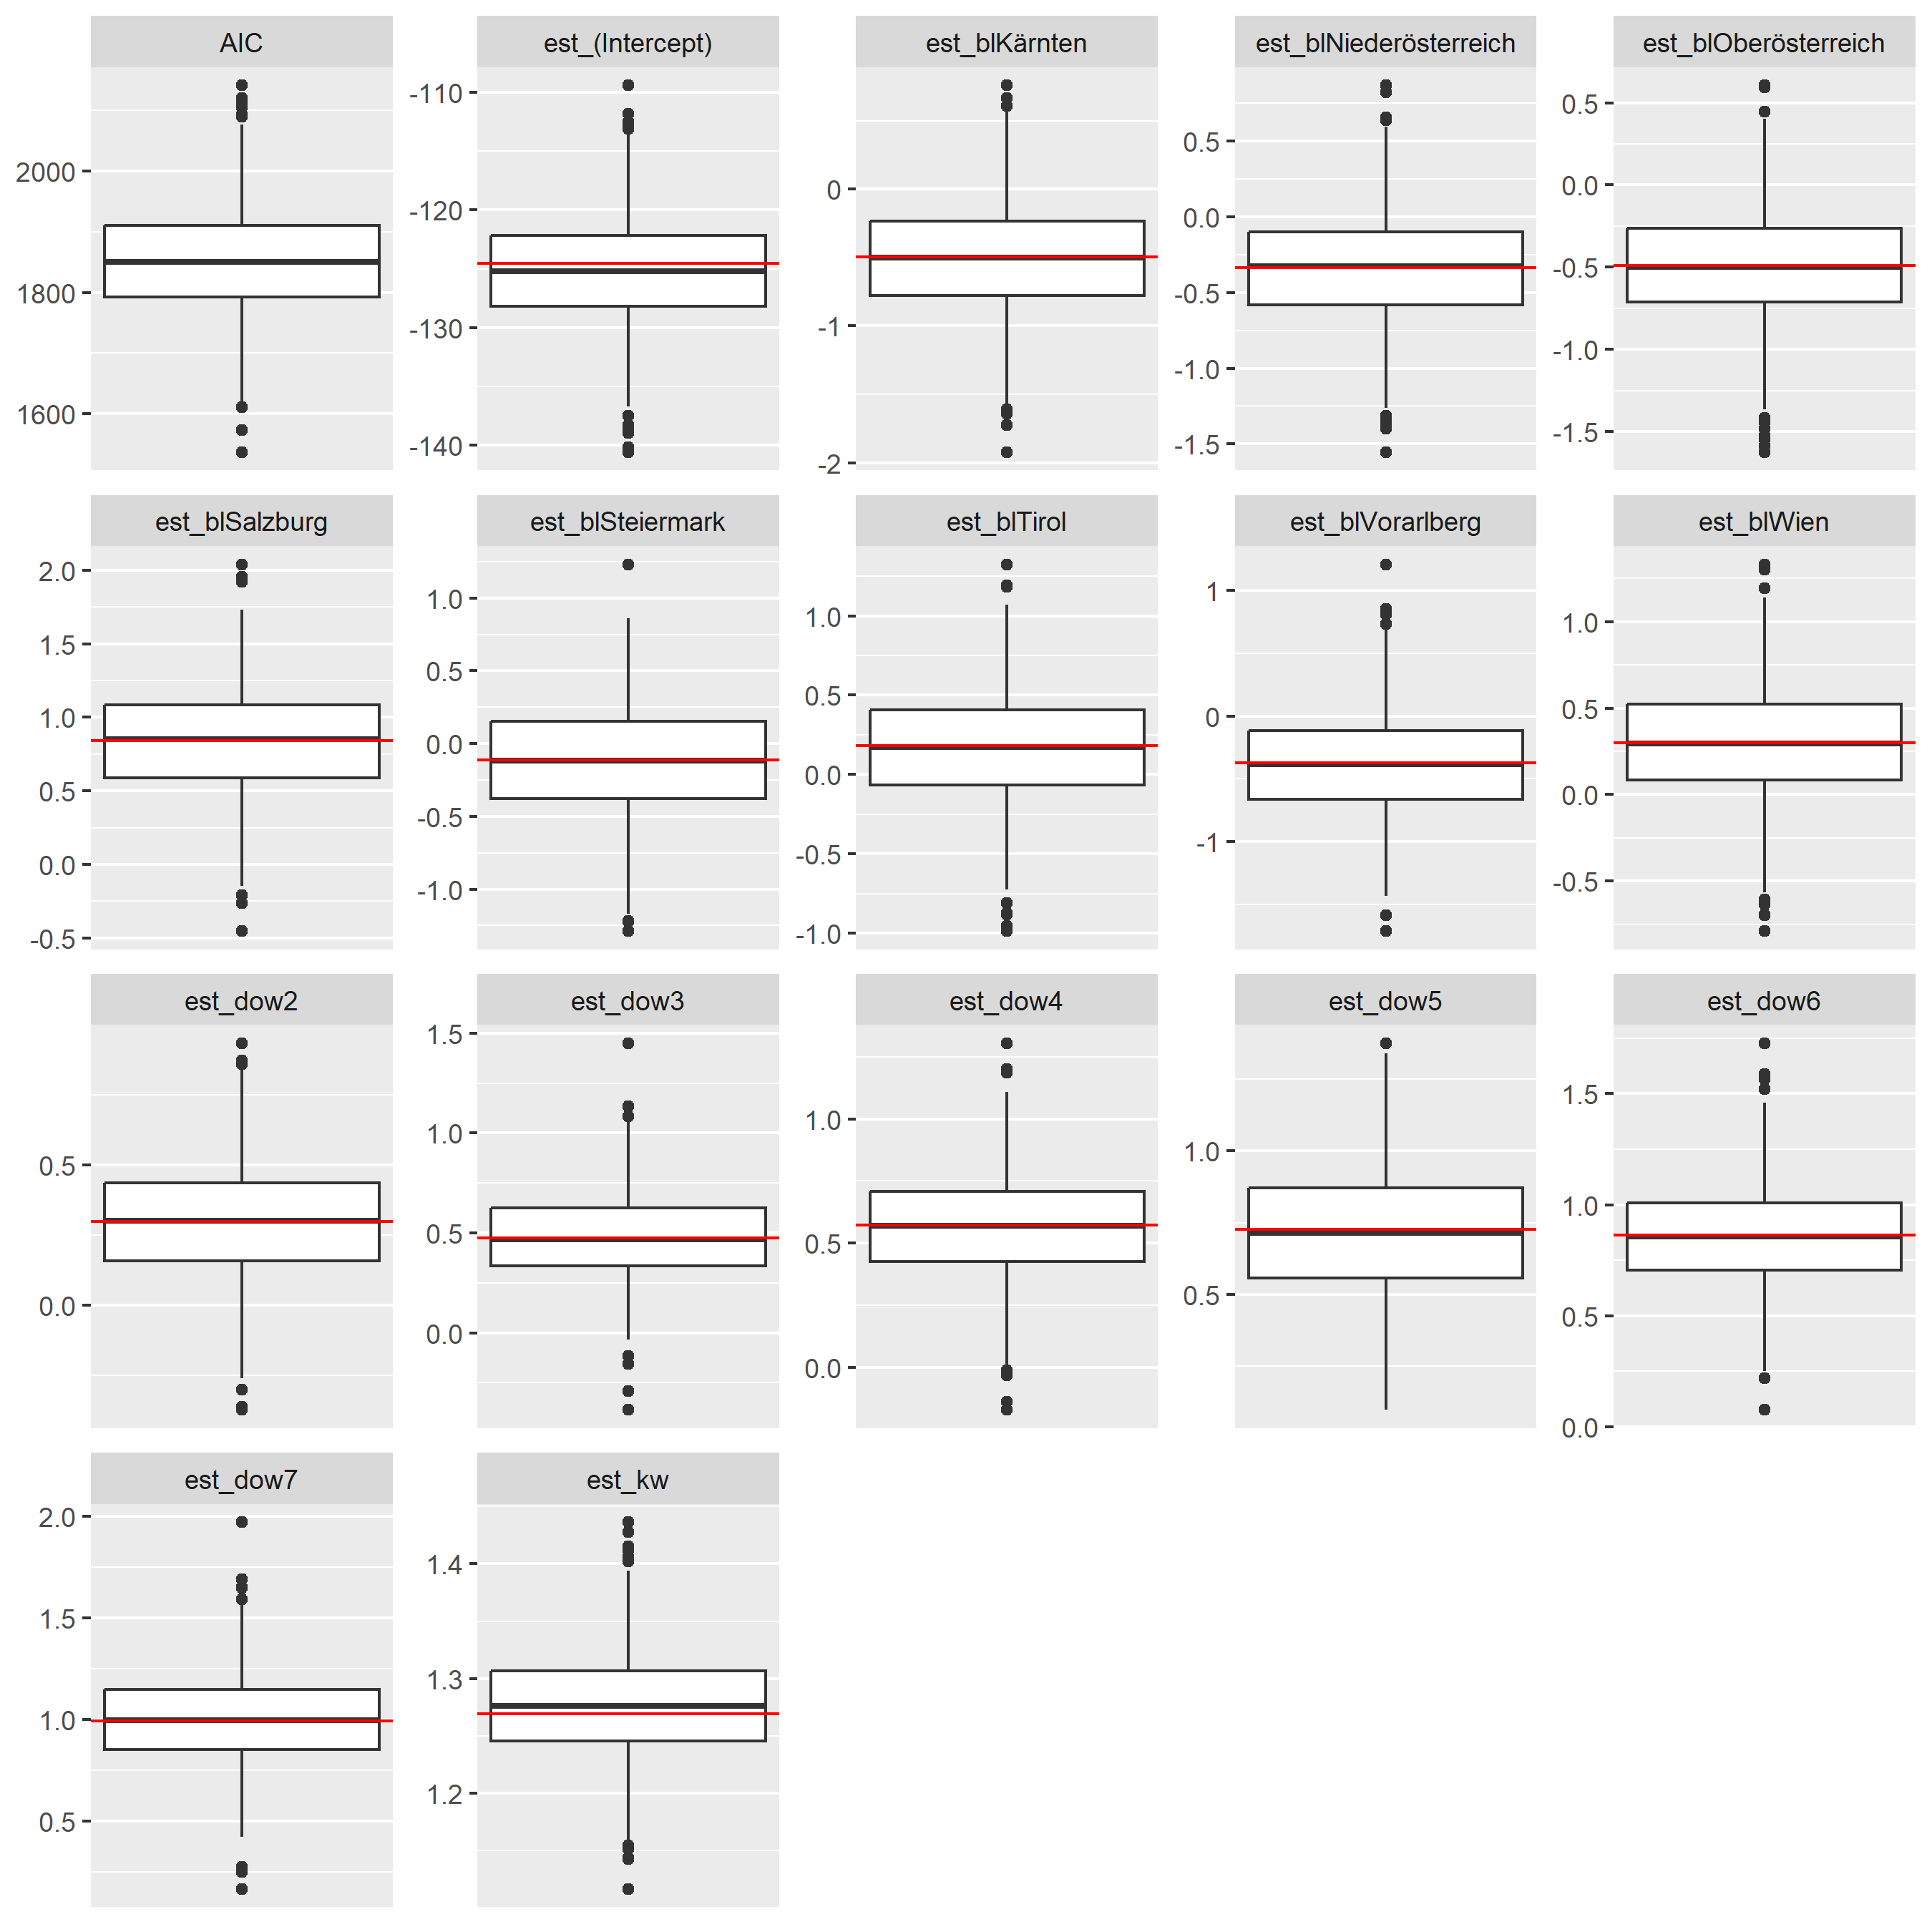
\includegraphics[height=0.8\textheight,keepaspectratio]{img/impute_omi_subset_samples_model_n501_estimates.png}
  \caption{Boxplots of model estimates of $r$ (being an N501Y case) based on 1,000 samples of size 23,658, 22.11.2021 to 14.02.2022. Results of the full dataset are shown as red lines.}
\end{figure}

\end{minipage}
\begin{minipage}{.30\textwidth}

\begin{itemize}
\item Median of model estimates are similar to full dataset
\item A single sample can yield extreme results
\item Standard deviation correlates with sample size (not shown)
\end{itemize}

\end{minipage}
\end{frame}

\begin{frame}{Why impute this data?}
\protect\hypertarget{why-impute-this-data}{}
\begin{figure}
  \centering
  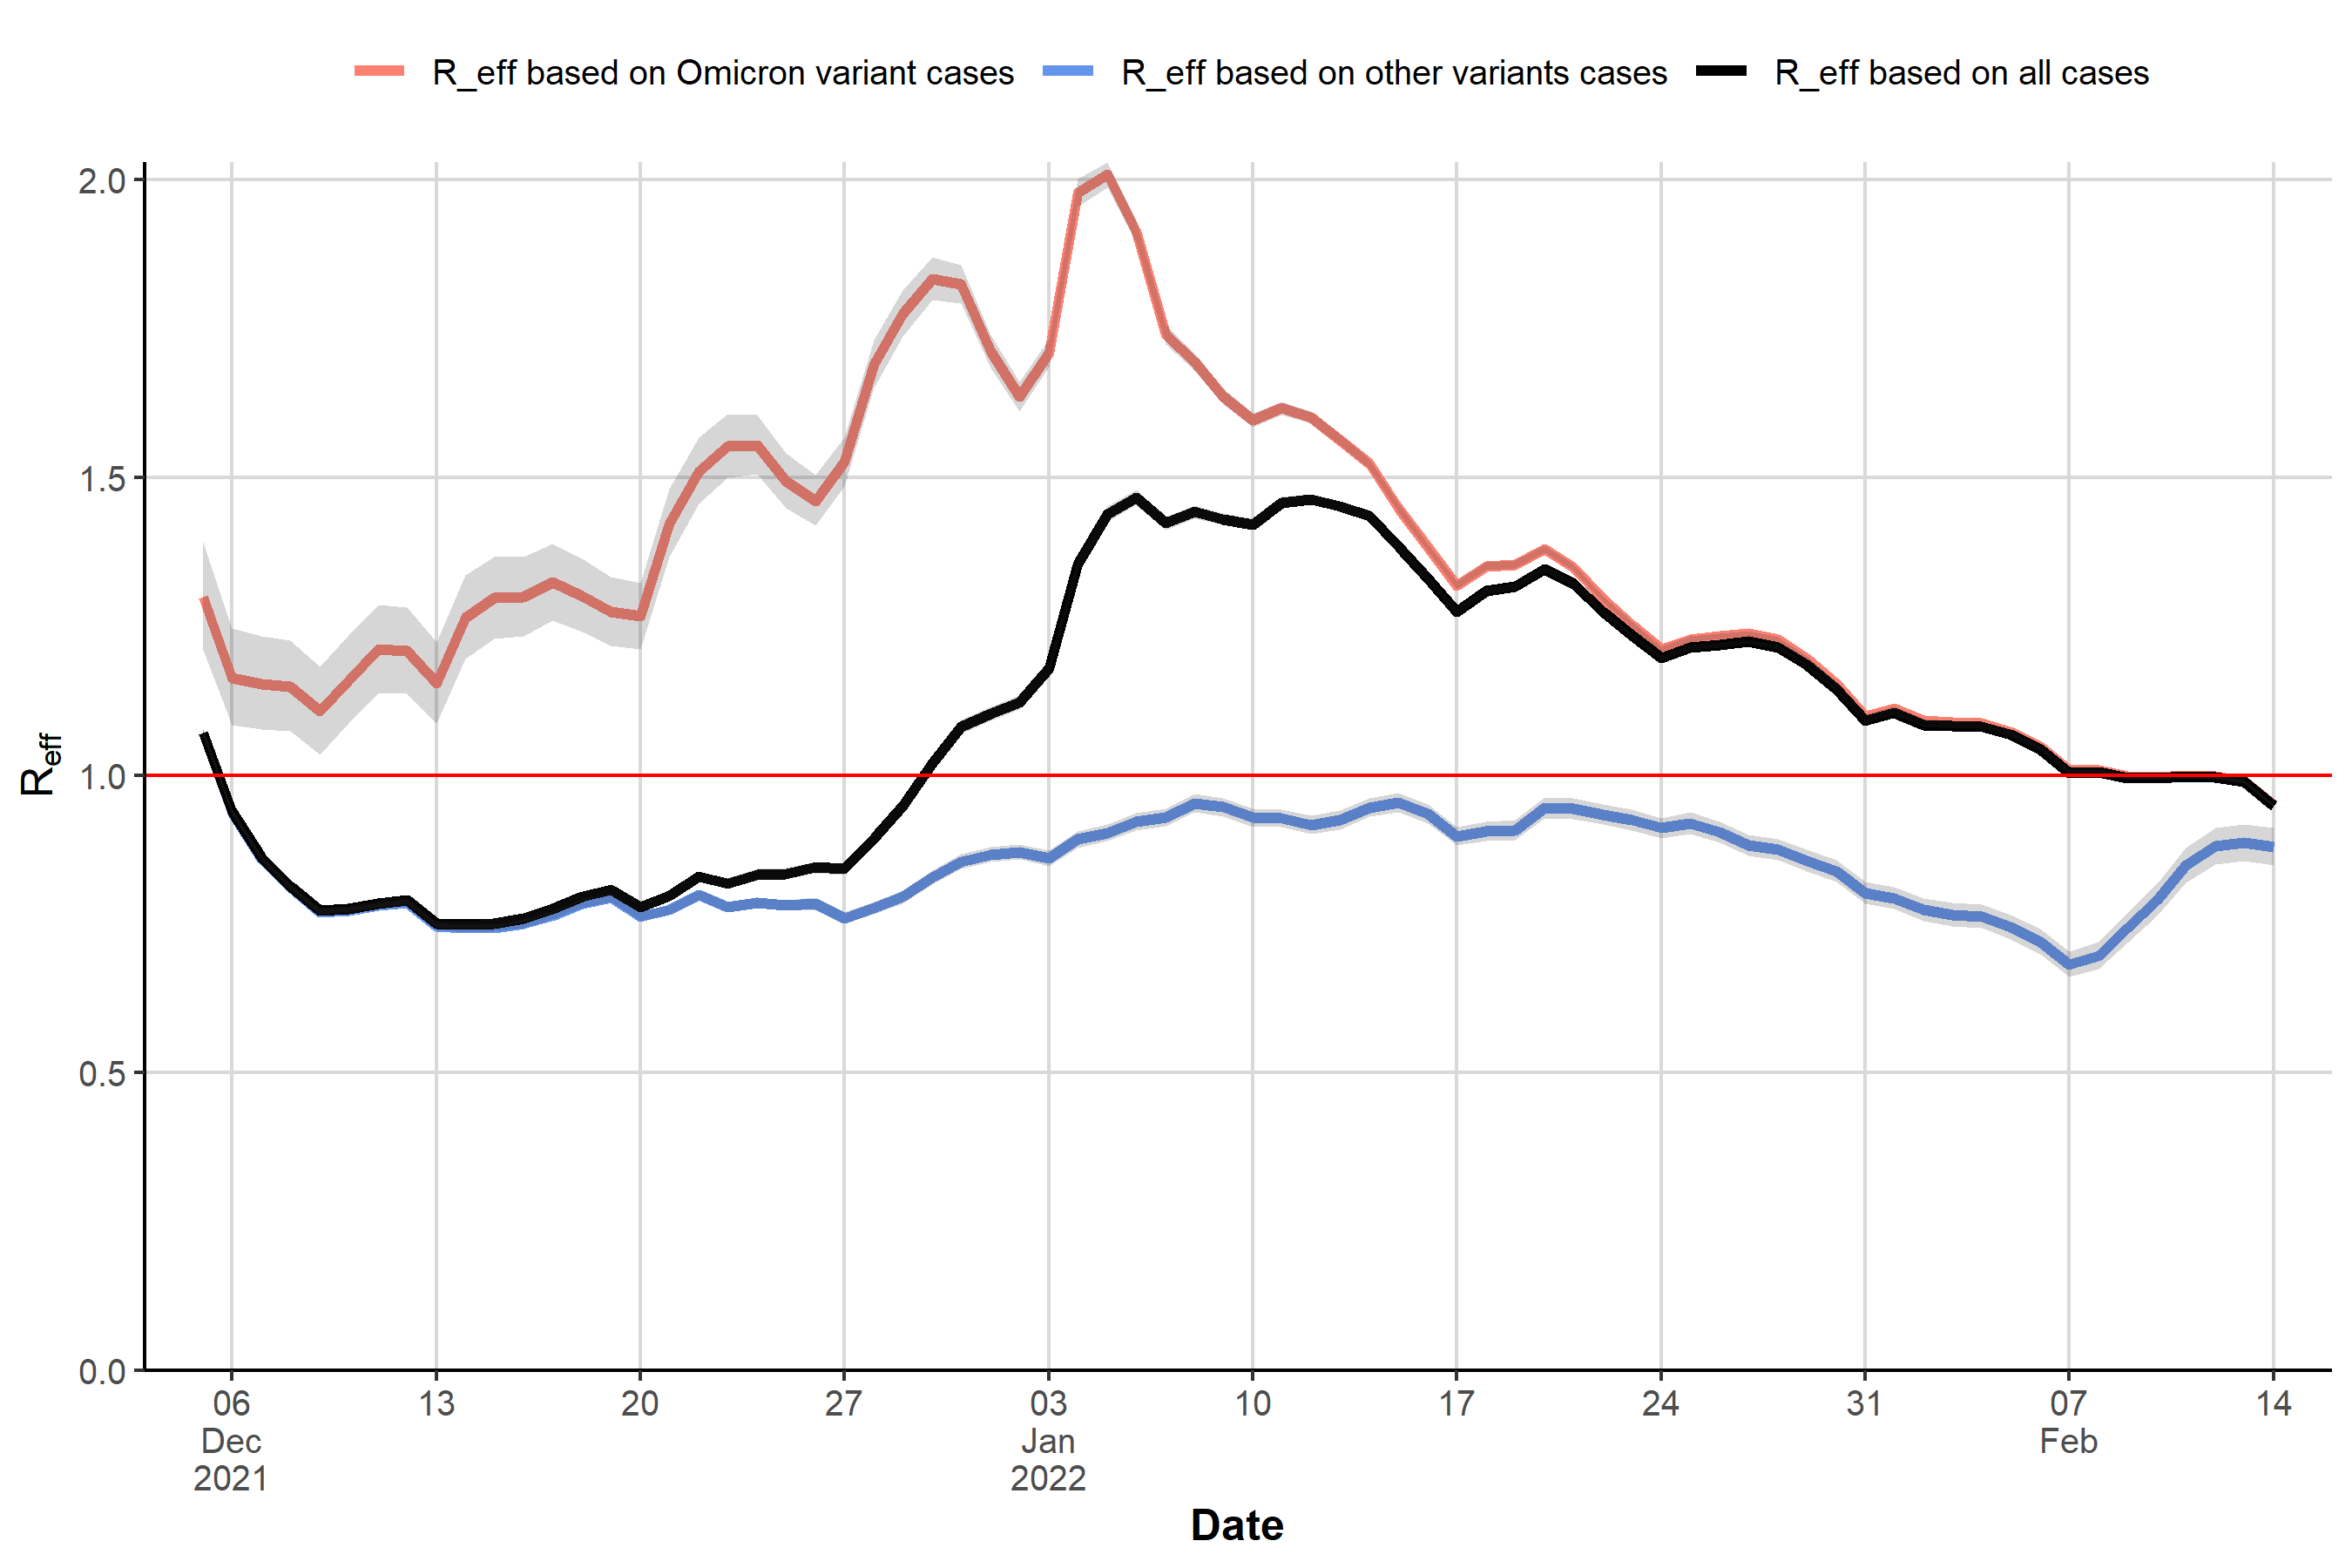
\includegraphics[height=0.8\textheight,keepaspectratio]{img/new_voc_omi_full_reff.png}
  \caption{Effective reproduction number based on date of lab diagnosis by (imputed) SARS-CoV-2 variant, Austria, 05.12.2021 to 14.02.2022}
\end{figure}
\end{frame}

\begin{frame}{Wrap up}
\protect\hypertarget{wrap-up}{}
\begin{itemize}
\item Statistical methods play an important role during outbreaks/pandemics.
\item We introduced methods to inform stakeholders and the public about key indicators ($SI$, $R_\mli{eff}$).
\item Impute missing data to analyse dynamics of new variants.
\end{itemize}

Other applications:

\begin{itemize}
\item Estimation of excess mortality
\item Vaccine effectiveness
\item Nowcasting and Forecasting
\end{itemize}
\end{frame}

\begin{frame}[noframenumbering,plain]{References}
\protect\hypertarget{references}{}
\scriptsize

\hypertarget{refs}{}
\begin{CSLReferences}{1}{0}
\leavevmode\vadjust pre{\hypertarget{ref-cori2013}{}}%
Cori, Anne, Neil M. Ferguson, Christophe Fraser, and Simon Cauchemez.
2013. {``A {New Framework} and {Software} to {Estimate Time}-{Varying
Reproduction Numbers During Epidemics}.''} \emph{American Journal of
Epidemiology} 178 (9): 1505--12.
\url{https://doi.org/10.1093/aje/kwt133}.

\leavevmode\vadjust pre{\hypertarget{ref-delignette-muller2015}{}}%
Delignette-Muller, Marie Laure, and Christophe Dutang. 2015.
{``Fitdistrplus: {An R Package} for {Fitting Distributions}.''}
\emph{Journal of Statistical Software} 64 (1): 1--34.
\url{https://doi.org/10.18637/jss.v064.i04}.

\leavevmode\vadjust pre{\hypertarget{ref-du2020}{}}%
Du, Zhanwei, Xiaoke Xu, Ye Wu, Lin Wang, Benjamin J. Cowling, and Lauren
Ancel Meyers. 2020. {``Early {Release} - {Serial Interval} of {COVID}-19
Among {Publicly Reported Confirmed Cases} - {Volume} 26, {Number}
6---{June} 2020 - {Emerging Infectious Diseases} Journal - {CDC}.''}
\url{https://doi.org/10.3201/eid2606.200357}.

\leavevmode\vadjust pre{\hypertarget{ref-nishiura2020}{}}%
Nishiura, Hiroshi, Natalie M. Linton, and Andrei R. Akhmetzhanov. 2020.
{``Serial Interval of Novel Coronavirus (2019-{nCoV}) Infections.''}
\emph{medRxiv}, February, 2020.02.03.20019497.
\url{https://doi.org/10.1101/2020.02.03.20019497}.

\leavevmode\vadjust pre{\hypertarget{ref-stasinopoulos2007}{}}%
Stasinopoulos, D. Mikis, and Robert A. Rigby. 2007. {``Generalized
{Additive Models} for {Location Scale} and {Shape} ({GAMLSS}) in {R}.''}
\emph{Journal of Statistical Software} 23 (1): 1--46.
\url{https://doi.org/10.18637/jss.v023.i07}.

\end{CSLReferences}
\end{frame}

\begin{frame}[noframenumbering,plain]{}
\protect\hypertarget{section}{}
\begin{center}
\begin{figure}
  \centering
  
\includegraphics[width=\textwidth,height=0.5\textheight,keepaspectratio]{img/Thank-you-word-cloud.jpg}
\end{figure}

Special Thanks to:\\
Ernst Stadlober\\
Team at AGES

\pause \Huge{\textbf{Any questions?}}
\vfill
\hfill {\scriptsize Contact: lukas.richter@ages.at}
\end{center}
\end{frame}

\begin{frame}[noframenumbering,plain]{Backup}
\protect\hypertarget{backup}{}
\begin{center}
\Huge\textbf{Backup slides}
\end{center}
\end{frame}

\begin{frame}[noframenumbering,plain]{PDFs of selected distributions}
\protect\hypertarget{pdfs-of-selected-distributions}{}
\begin{itemize}
\item gamma distribution: $p(x;\alpha,\beta):=\frac{x^{\alpha-1}e^{-\beta x} \beta^{\alpha}}{\Gamma(\alpha)}, x>0, \alpha>0, \beta>0.$

\item lognormal distribution: $p(x;\mu,\sigma)=\frac{1}{x\sigma\sqrt{2\pi}}\exp\left(-\frac{(\ln x - \mu)^2}{2\sigma^2}\right), x>0, \sigma > 0$

\item exponential distribution: $p(x;\lambda)=\lambda e^{-\lambda x}, x\geq 0, \lambda>0.$

\item Weibull distribution: $p(x;k,\lambda)=\frac{k}{\lambda} \left(\frac{x}{\lambda}\right)^{k-1} e^{{-(x/\lambda)}^k}, x\geq 0, k>0, \lambda>0.$

\end{itemize}
\end{frame}

\begin{frame}[noframenumbering,plain]{SI estimates, 06.09.2020 --
17.05.2021 (Alpha variant period)}
\protect\hypertarget{si-estimates-06.09.2020-17.05.2021-alpha-variant-period}{}
\begin{table}

\caption{Fitted parameters, mean, standard deviation, 95\% confidence intervals and AIC.}
\centering
\begin{tabular}{llrlrrrr}
\toprule
distribution & parameter & value & mean & mean 95\% CI & sd & sd 95\% CI & AIC\\
\midrule
 & $\alpha$ & 3.38 &  &  &  &  & \\

\multirow{-2}{*}{\raggedright\arraybackslash gamma} & $\beta$ & 1.00 & \multirow{-2}{*}{\raggedright\arraybackslash 3.37} & \multirow{-2}{*}{\raggedleft\arraybackslash 3.15--3.60} & \multirow{-2}{*}{\raggedleft\arraybackslash 1.83} & \multirow{-2}{*}{\raggedleft\arraybackslash 1.64--2.03} & \multirow{-2}{*}{\raggedleft\arraybackslash 963.3}\\
\cmidrule{1-8}
 & $\mu$ & 1.06 &  &  &  &  & \\

\multirow{-2}{*}{\raggedright\arraybackslash lnorm} & $\sigma$ & 0.56 & \multirow{-2}{*}{\raggedright\arraybackslash 3.38} & \multirow{-2}{*}{\raggedleft\arraybackslash 3.12--3.62} & \multirow{-2}{*}{\raggedleft\arraybackslash 2.05} & \multirow{-2}{*}{\raggedleft\arraybackslash 1.74--2.37} & \multirow{-2}{*}{\raggedleft\arraybackslash\bf 954.2}\\
\cmidrule{1-8}
exp & $\lambda$ & 0.30 & 3.37 & 2.97--3.74 & 3.37 & 2.97--3.74 & 1,109.2\\
\cmidrule{1-8}
 & $k$ & 1.84 &  &  &  &  & \\

\multirow{-2}{*}{\raggedright\arraybackslash Weibull} & $\lambda$ & 3.81 & \multirow{-2}{*}{\raggedright\arraybackslash 3.39} & \multirow{-2}{*}{\raggedleft\arraybackslash 3.15--3.62} & \multirow{-2}{*}{\raggedleft\arraybackslash 1.91} & \multirow{-2}{*}{\raggedleft\arraybackslash 1.73--2.08} & \multirow{-2}{*}{\raggedleft\arraybackslash 986.1}\\
\bottomrule
\end{tabular}
\end{table}
\end{frame}

\begin{frame}[noframenumbering,plain]{\(R_\mli{eff}\), Cori Method,
Bayesian inference I}
\protect\hypertarget{r_mlieff-cori-method-bayesian-inference-i}{}
\begin{itemize}
\item As prior for $R_{t,\tau}$ we choose a Gamma distribution and we get:
\begin{align}
  p(R_{t,\tau};a,b)=p(R_{t,\tau}):=\frac{R_{t,\tau}^{a-1}e^{-R_{t,\tau}/b}}{b^a\Gamma(a)}, R_{t,\tau}>0, a>0, b>0 \label{eq:p1}
\end{align}
\item The likelihood is given by
\begin{align}
  p(\boldsymbol{y};R_{t,\tau}) = \prod_{i=t-\tau+1}^t (R_{t,\tau} d_i)^{y_i} \exp\left(-R_{t,\tau} d_i\right)\frac{1}{y_i!} \label{eq:p2}
\end{align}
with $d_i:=\sum_{s=1}^i y_{i-s}w_s$
\end{itemize}
\end{frame}

\begin{frame}[noframenumbering,plain]{\(R_\mli{eff}\), Cori Method,
Bayesian inference II}
\protect\hypertarget{r_mlieff-cori-method-bayesian-inference-ii}{}
\begin{itemize}
\item Posterior:
\begin{align}
  p(R_{t,\tau};\boldsymbol{y}) = \frac{p(\boldsymbol{y};R_{t,\tau})p(R_{t,\tau})}{\int p(\boldsymbol{y};R_{t,\tau})p(R_{t,\tau})\, d\, R_{t,\tau}} \label{eq:p3}
\end{align}
\item Plug \eqref{eq:p1} and \eqref{eq:p2} into \eqref{eq:p3} and reformulate the expression:
\begin{align*}
  p(R_{t,\tau};\boldsymbol{y}) = R_{t,\tau}^{a+\sum_{i=t-\tau+1}^t y_i - 1} \exp\left(-R_{t,\tau}\left(\frac{1}{b} + \sum_{i=t-\tau+1}^t d_i \right)\right) k(\boldsymbol{y},t,a,b),
\end{align*}
with
\begin{align*}
k(\boldsymbol{y},t,a,b) = \prod_{i=t-\tau+1}^t \frac{d_i^{y_i} c}{y_i! b^a \Gamma(a)}
\end{align*}
\item $\Rightarrow p(R_{t,\tau};\boldsymbol{y})$ is proportional to
\begin{align*}
  p(R_{t,\tau};\boldsymbol{y}) \propto R_{t,\tau}^{a+\sum_{i=t-\tau+1}^t y_i - 1} \exp\left(-R_{t,\tau}\left(\frac{1}{b} + \sum_{i=t-\tau+1}^t d_i \right)\right) \frac{\frac{1}{b}+\sum_{i=t-\tau+1}^t d_i}{\Gamma(a+\sum_{i=t-\tau+1}^t y_i)}
\end{align*}
\end{itemize}
\end{frame}

\begin{frame}[noframenumbering,plain]{\(R_\mli{eff}\), Cori Method,
Bayesian inference III}
\protect\hypertarget{r_mlieff-cori-method-bayesian-inference-iii}{}
\hfsetfillcolor{green!10}
\hfsetbordercolor{green!50!black}
\begin{itemize}
\item It follows that
\begin{align}
  R_{t,\tau} \sim \text{Gamma}\left(a+\sum_{i=t-\tau+1}^t y_i, \frac{1}{\frac{1}{b} + \sum_{i=t-\tau+1}^t d_i}\right)
\end{align}
\item The estimate of $R_\mli{eff}$ at day $t$ and based on $\tau$ days is the mean of $R_{t,\tau}$ and is given as
\begin{align*}
  \tikzmarkin{a}(0.05,-0.6)(-0.05,0.65)\hat{R}_{t,\tau}\tikzmarkend{a} &= \frac{a+\sum_{i=t-\tau+1}^t y_i}{\frac{1}{b} + \sum_{i=t-\tau+1}^t d_i} \\
  &=\tikzmarkin{c}(0.05,-0.6)(-0.05,0.65) \frac{a+\sum_{i=t-\tau+1}^t y_i}{\frac{1}{b} + \sum_{i=t-\tau+1}^t \sum_{s=1}^i y_{i-s}w_s}\tikzmarkend{c}
\end{align*}
\end{itemize}
\end{frame}

\end{document}
